% Se compila con XeLaTeX; hacen falta varias pasadas para que se resuelvan las referencias.
\documentclass[11pt,a4paper]{article}
\usepackage{fontspec}
\IfFontExistsTF{texgyrepagella-regular.otf}
 {\setmainfont{texgyrepagella}[Extension=.otf,UprightFont=*-regular,BoldFont=*-bold,
   ItalicFont=*-italic,BoldItalicFont=*-bolditalic]}
 {\IfFontExistsTF{Palatino Linotype}{\setmainfont{Palatino Linotype}}{\setmainfont{Latin Modern Roman}}}
\linespread{1.05}
% Con babel-spanish instalado (MiKTeX, TeX Live completo) se usa la opción clásica; si falta,
% se carga el locale español de babel sin patrones de guionado y los cortes de palabra se
% toman de guionado.tex.
\IfFileExists{spanish.ldf}
 {\usepackage[spanish,es-noshorthands,es-nodecimaldot,es-tabla]{babel}}
 {\usepackage{babel}\babelprovide[import,main,hyphenrules=nohyphenation]{spanish}% Puntos de corte de las palabras del artículo según la división silábica de la Ortografía de
% la lengua española (RAE y ASALE, 2010); no se separan vocales contiguas. Sólo se usa cuando
% la instalación de TeX no trae los patrones de guionado del español (véase preambulo.tex).
\babelhyphenation[spanish]{
ab-so-lu-ta ab-so-lu-ta-men-te ab-so-lu-tos ab-sor-be ab-sor-be-do-res ab-sor-be-dor
ab-sor-ber-lo aba-jo abier-to abier-tos ac-ti-va ac-ti-vas ac-ti-vi-dad ac-ti-vo ac-ti-vos
ac-túa ac-túan acer-ca aco-ta aco-ta-ción aco-ta-da aco-ta-das aco-ta-do aco-ta-dos
acu-mu-la-da acu-mu-la-do acu-mu-lan ad-mi-si-ble ad-mi-si-bles ad-mi-ta ad-mi-te ad-mi-ten
ad-mi-tir ad-ver-sa-ria-les ade-más afec-ta afir-ma afir-ma-cio-nes afir-ma-ción agre-ga-do
agru-pa-mos aho-ra ais-la-da ajus-tar al-can-ce al-can-za al-gún al-re-de-dor al-te-ra
al-ter-na-ti-va-men-te alea-to-ria alea-to-rio alea-to-rios ali-men-ta alu-de am-bas am-bos
an-chu-ra an-te-rio-res an-te-rior an-tes an-ti-dia-go-na-les an-ti-dia-go-nal ana-li-za
ana-lí-ti-ca ana-lí-ti-cas anu-la anu-lan anun-cia-da aná-li-sis aná-lo-gas apa-re-ce
apa-ri-ción apar-ta-dos apli-ca apli-ca-da apli-ca-do apli-ca-mos apli-car apli-car-la
apo-ya apor-tan apro-ve-chan apro-xi-ma apro-xi-ma-ción apén-di-ce ar-bi-tra-rias ar-chi-vo
ar-gu-men-to ar-ti-fi-cial ar-tí-cu-lo ar-xiv-per-fil aris-ta aris-tas ase-gu-ra asi-mis-mo
asig-na asig-na-do asig-na-mos asin-tó-ti-ca asin-tó-ti-ca-men-te asin-tó-ti-co aso-cia-dos
ata-ca ata-ca-do ata-can ata-que ata-ques au-men-ta au-men-ta-do au-xi-lia-res aun-que
avan-za axio-mas aña-de aña-den aña-dir ba-lan-ce bas-ta bas-ta-ría bi-la-te-ra-les
bi-na-ria bi-yec-ción blan-co blan-cos blo-que bo-rra bo-rra-do bo-rra-dos bo-rrar bor-de
bor-des bus-ca-da ca-bría ca-de-na ca-pas ca-rac-te-ri-za ca-re-ce ca-si-lla ca-si-llas
ca-sos cal-cu-la-do cam-bia cam-bian cam-biar cam-bio cam-bios can-ce-la can-ce-la-ción
can-ce-lan can-ce-lar-se can-di-da-ta can-di-da-tas car-te-sia-na car-te-sia-nas ce-ros
ce-rra-do cen-tros cer-ca cer-ca-no cer-ti-fi-ca-ción cer-ti-fi-ca-da cer-ti-fi-ca-do
cie-rre cin-co cir-cu-la-ri-dad cla-ve co-cien-te co-cien-tes co-de-gra-do co-lo-ca
co-lo-ca-cio-nes co-lo-ca-ción co-lo-ca-das co-lo-ca-do co-lo-ca-mos co-lo-can co-lo-car
co-lo-car-la co-lo-res co-lor co-lum-na co-lum-nas co-mu-nes co-mún co-nec-tan co-no-ce-mos
co-ro-la-rio co-rres-pon-de co-rres-pon-den co-rres-pon-dien-te co-tas co-te-jar
coe-fi-cien-te coe-fi-cien-tes coer-ci-vi-dad coin-ci-de com-bi-na-ción com-bi-na-to-ria
com-pa-ra com-pa-ra-ción com-pa-ran-do com-pa-rar com-pa-ti-ble com-pa-ti-bles com-pac-to
com-pac-tos com-par-ten com-pen-sa-ción com-pen-sa-dor com-pi-la-ción com-pi-la-dos
com-pi-lar-lo com-ple-men-ta-rio com-ple-ta com-ple-ta-bi-li-dad com-ple-ta-bles
com-ple-ta-cio-nes com-ple-ta-ción com-ple-ta-do com-ple-tan com-ple-tar com-ple-tar-se
com-ple-tas com-ple-ti-tud com-ple-to com-po-si-ción com-pro-ba-ción com-pro-bar com-prue-ba
con-ca-vi-dad con-cen-tra con-cen-tra-ción con-cen-tran con-cen-tre con-cier-ne
con-clu-sio-nes con-clu-sión con-di-cio-na con-di-cio-na-da con-di-cio-nal-men-te
con-di-cio-nar con-di-ción con-ge-la-mos con-ge-lan con-jun-ta con-jun-to con-mu-ta-cio-nes
con-se-cu-ti-vas con-se-cuen-cia con-se-cuen-cias con-ser-va con-ser-va-do-ra
con-ser-va-do-ras con-ser-van con-ser-ve con-si-de-rar con-si-de-re-mos con-si-guien-te
con-sis-te con-ta-do con-ta-do-res con-ta-dor con-ta-mos con-tar con-te-ni-da con-teo
con-teos con-ti-nua con-ti-nua-men-te con-ti-nuas con-ti-nui-dad con-ti-nuo con-tie-ne
con-tra-di-ce con-tri-bu-ción con-tro-la con-tro-la-da con-tro-lan con-tro-lar con-trol
con-ver-ge con-ver-gen con-ver-gen-cia con-vier-te cons-tan-te cons-tan-tes cons-tru-ye
cons-tru-yen cons-truc-ción cons-trui-da cons-trui-das cons-truir coor-de-na-da
coor-de-na-das cor-che-tes cor-ta cor-tan cor-te cre-ce cre-cer cre-cien-te cre-cien-tes
crea-do crez-ca cru-ce cru-ces cu-bier-to cu-bier-tos cu-bre cu-yas cu-yos cua-dra-do
cua-dra-tu-ra cua-dra-tu-ras cua-drá-ti-ca cua-drí-cu-la cua-ter-nas cua-tro cual-quie-ra
cual-quier cuan-do cuen-ta cuen-tas cues-ta cum-ple cum-plen có-di-go cón-ca-va cón-ca-vo
da-dos da-mos da-tos de-ci-ma-les de-ci-mal de-cir de-du-ce de-du-cir de-fi-ne de-fi-nen
de-fi-ni-cio-nes de-fi-ni-ción de-fi-ni-mos de-jan de-jar de-lan-te de-mos-tra-ción
de-mos-tra-da de-mos-tra-do de-mos-tra-mos de-mues-tra de-mues-tran de-más
de-no-mi-na-do-res de-no-mi-na-dor de-no-ta de-no-ta-mos de-no-tan de-no-te-mos de-pen-de
de-pen-den de-pen-den-cia de-pen-der de-re-cha de-ri-va de-ri-va-bi-li-dad de-ri-va-da
de-ri-va-das de-ri-van-do de-ri-vas de-sac-ti-va de-sac-ti-van de-si-gual-da-des
de-si-gual-dad de-sig-na de-te-ni-das de-te-ni-do de-ter-mi-na de-ter-mi-na-da
de-ter-mi-na-do de-ter-mi-nis-ta de-ter-mi-nis-tas de-ter-mi-nís-ti-ca-men-te de-tie-nen
den-si-da-des den-si-dad des-cri-be des-cri-ben des-cri-ta des-crip-cio-nes des-crip-ción
des-de des-ha-ce des-ha-cer des-pués des-ti-no des-ti-nos des-tru-ye des-truir
des-via-cio-nes di-fe-ren-cia di-fe-ren-cia-les di-fe-ren-cias di-fie-re di-fie-ren
di-men-sión di-ná-mi-ca di-re-mos di-rec-cio-nes di-rec-ción di-rec-ta di-rec-ta-men-te
di-rec-tas di-rec-to di-rec-tos di-ver-gen-cia di-vi-de di-vi-di-do di-vi-dien-do di-vi-dir
dia-go-na-les dia-go-nal dia-go-nal-men-te die-ci-séis dis-cre-ta dis-cre-tas
dis-cre-ti-za-ción dis-cre-to dis-cu-sión dis-po-ni-bi-li-dad dis-po-ni-ble dis-po-ni-bles
dis-tin-ción dis-tin-ta dis-tin-tas dis-tin-to dis-tin-tos dis-tri-bu-ción dis-tri-bu-ye
dis-tri-bui-da do-ble do-bles do-mi-nio do-mi-nios don-de du-ran-te dua-li-dad dé-bil
dé-bil-men-te dón-de ecua-cio-nes ecua-ción edi-to-rial efec-ti-vas efec-to ejem-plo
ejem-plos ela-bo-rar ele-gi-das ele-gi-do ele-gi-dos ele-gi-mos ele-gi-re-mos ele-gir
ele-men-tal ele-men-tos elec-cio-nes elec-ción eli-ge eli-gen eli-gien-do eli-mi-na
eli-mi-na-do eli-mi-na-dos eli-mi-nar em-pa-re-ja-mien-to em-pa-re-jan-do em-pal-me
em-pí-ri-ca en-cuen-tre en-la-ce en-te-ro en-te-ros en-ten-der en-ton-ces en-tre en-tro-pía
en-tró-pi-ca enu-me-ra-ción enun-cia enun-cia-do enun-cia-dos equi-va-le equi-va-len-cia
erro-res es-ca-la es-ca-lar es-ca-lo-na-da es-ca-lo-na-do es-ca-lo-na-dos es-co-ge es-cri-be
es-cri-ben es-cri-bi-mos es-cri-bien-do es-pa-cial es-pa-cio es-pe-ra-do es-pe-ran-za
es-pe-ran-zas es-pí-ri-tu es-ta-ble-ce es-ta-cio-na-rie-dad es-ta-do es-ta-rá es-ta-rán
es-tas es-ti-ma-cio-nes es-ti-ma-ción es-ti-mar es-tos es-truc-tu-ra es-tu-dia es-tu-dia-mos
es-tu-dian es-tu-diar es-tán es-tén eva-lua-da eva-lua-do eva-luar eva-lúa even-to even-tos
evi-ta evo-lu-ción ex-ce-den ex-cep-cio-na-les ex-cep-cio-nes ex-cep-ción
ex-clu-si-va-men-te ex-clu-sio-nes ex-clu-sión ex-clu-yen ex-clui-das ex-clui-dos
ex-haus-ti-va ex-pe-ri-men-to ex-pli-ca ex-plí-ci-ta ex-plí-ci-tas ex-plí-ci-to
ex-plí-ci-tos ex-po-nen-cial ex-pre-sa ex-pre-sar ex-pre-sión ex-ten-di-da ex-ten-sio-nes
ex-ten-sión ex-tien-de ex-tien-den ex-tra-po-la-ción ex-trac-tos ex-tre-mal ex-tre-mas
ex-tre-mo exac-ta exac-ta-men-te exac-tos exi-ge exi-gi-ría exi-to-sa exis-te exis-ten
exis-ten-cia exis-ten-cial fa-lla fa-llo fa-mi-lia fa-mi-lias fac-to-res fac-to-ri-za
fac-to-ri-za-ción fac-tor fal-ta fal-tan fi-bra fi-bras fi-gu-ra fi-gu-ras fi-ja-da
fi-ja-mos fi-jan fi-jan-do fi-jas fi-je-mos fi-jos fi-las fi-na-les fi-nal fi-nal-men-te
fi-ni-to fi-ni-tud fic-ti-cio fic-ti-cios fil-tro fle-chas for-ma for-ma-li-za-ción
for-ma-li-za-do for-ma-li-za-dos for-mal for-man frac-ción fran-ja fre-cuen-cia fren-te
fue-ra fuen-te fuen-tes fun-cio-na fun-cio-nal fun-cio-nes fun-ción fí-si-ca-men-te
fí-si-cas fí-si-co fí-si-cos fór-mu-la ge-ne-ra ge-ne-ra-do ge-ne-ra-dor ge-ne-ra-les
geo-me-tría geo-mé-tri-ca gra-dien-te gra-do gra-dos gran-de gran-des ha-bi-tual ha-ble-mos
ha-bía ha-ce-mos ha-cia ha-llar has-ta he-mos he-re-da he-rra-mien-ta he-rra-mien-tas
hes-sia-no heu-rís-ti-ca heu-rís-ti-ca-men-te hi-per-gra-fo hi-pó-te-sis ho-ri-zon-te
ho-ri-zon-tes hue-co hue-cos iden-ti-dad iden-ti-fi-ca iden-ti-fi-ca-ción iden-ti-fi-ca-mos
iden-ti-fi-can iden-ti-fi-car idén-ti-ca igua-les igual-dad ili-mi-ta-da ilus-tra-ción
im-pli-ca im-po-si-ble ima-gen in-ci-de in-clu-sión in-clu-so in-clu-ye in-clui-da
in-clui-do in-clui-dos in-clui-mos in-cre-men-tos in-de-pen-den-cia in-de-pen-dien-te
in-de-pen-dien-te-men-te in-de-pen-dien-tes in-de-xa-mos in-de-xan in-di-ca in-di-ca-ción
in-di-ca-do-res in-di-ca-dor in-di-can in-di-car in-di-vi-dua-les in-du-cen in-du-ci-das
in-fe-rior in-fe-rior-men-te in-fi-ni-ta in-for-ma-ción in-for-me in-me-dia-to
in-ser-cio-nes in-ser-ción in-ser-ta in-te-gra in-te-gra-bi-li-dad in-te-gra-do
in-te-gra-les in-te-gral in-te-gran in-te-gran-do in-te-grar in-te-li-gen-cia in-te-rior
in-ten-tar in-ter-pre-ta-ción in-ter-sec-ción in-ter-va-lo in-ter-va-los in-ter-vie-ne
in-tro-duc-ción in-ver-sa in-ver-sas in-ver-so in-ver-sos in-ver-tir in-ver-tir-se
inac-ti-vo ini-cial ini-cio ins-tan-te iso-me-tría ite-ra-do ja-co-bia-no je-rar-quía
jun-tas jun-to lar-go le-ga-les le-gal le-jos le-mas le-van-tar le-yes li-bre li-bres
li-neal lis-ta lla-ma-mos lla-ma-re-mos lle-gan lle-no lle-va lle-van lo-ga-rít-mi-co
lo-ga-rít-mi-cos lon-gi-tud lu-gar lue-go lí-mi-te lí-mi-tes lí-nea lí-neas ló-gi-ca ma-llas
ma-ne-ra ma-sas ma-xi-ma-li-dad ma-xi-mi-za ma-xi-mi-za-dor man-tie-ne mar-ca mar-cas
mar-gi-na-les mar-gi-nal mar-tin-ga-la mar-tin-ga-las me-di-ble me-di-da me-dia me-dian-te
me-dias me-dio me-jo-ra me-nor me-nos miem-bro miem-bros mien-tras mis-ma mis-mas mis-mo
mis-mos mix-tos mo-de-lo mo-de-ra-dos mo-men-to mo-ver mo-vi-mien-to mue-re muer-te mues-tra
mues-tran mues-trear mul-ti-pli-can-do mul-ti-pli-car má-xi-mo mé-to-do mó-du-lo mó-du-los
múl-ti-plo na-ci-mien-to na-ci-mien-tos ne-ce-si-ta ne-ce-si-ta-mos ne-ga-ti-va
ne-ga-ti-vi-dad neu-tro nin-gu-na nin-gún no-ta-ción no-ve-dad nor-ma nor-ma-li-za-ción
nor-ma-li-za-do nor-ma-li-za-do-res nor-ma-li-za-dor nor-ma-li-za-dos nor-ma-li-zan nu-los
nu-me-ra-mos nu-mé-ri-ca nu-mé-ri-co nu-mé-ri-cos nue-va nue-vas nue-vo nue-vos nues-tra
nú-cleo nú-me-ro ob-je-ti-vo ob-ser-va ob-ser-va-bles ob-ser-va-ción ob-te-ne-mos ob-te-ner
ob-te-ni-das ob-te-ni-do ob-te-ni-dos ob-tie-ne ob-tie-nen ob-tu-vo ocu-pa ocu-pa-da
ocu-pa-das ocu-pa-do ocu-pa-rían ocu-pan ocu-par ocu-rre ofre-ce omi-ti-mos op-ti-mi-za-ción
ope-ra-cio-nes ope-ra-ción ope-ra-do-res ope-ra-dor or-de-na-do or-de-na-dos or-den
or-di-na-ria or-di-na-rias or-di-na-rio or-ga-ni-zar or-to-go-na-li-dad ori-gi-na-les
ori-gi-nal orien-ta-cio-nes pa-la-bra pa-la-bras pa-pel pa-ra-da pa-ra-me-tri-za-da
pa-ra-mé-tri-ca pa-re-jas pa-res pa-rá-me-tro pa-rá-me-tros pa-sa-mos pa-san pa-sar pa-sos
pa-tro-nes pa-trón par-cial par-te par-ti-cu-lar par-ti-mos par-ti-to pe-di-do pe-que-ña
pe-que-ño pe-que-ños pe-sos pen-dien-te pen-dien-tes per-der per-fec-to per-fi-les per-fil
per-ma-ne-ce per-ma-ne-cen per-mi-te per-mi-ti-rá per-mi-tien-do per-mu-ta-ción
per-mu-to-nes per-mu-tón pie-za pie-zas po-de-mos po-drían po-ne-mos po-si-ble po-si-bles
po-si-cio-nes po-si-ción po-si-ti-va po-si-ti-vas po-si-ti-vi-dad po-si-ti-vo po-si-ti-vos
pon-de-ra-da pon-de-ra-das pon-de-ra-dos por-que pre-ce-de pre-ci-sa pre-gun-ta
pre-li-mi-na-res pre-pa-rar pre-ten-de pre-via-men-te pre-vio pre-vios prea-sig-na pri-me-ra
pri-me-ro pri-mer prin-ci-pa-les prin-ci-pal pro-ba-bi-li-da-des pro-ba-bi-li-dad pro-ba-mos
pro-bar pro-bar-la pro-ble-ma pro-ble-mas pro-ce-de pro-ce-den pro-ce-sa-mien-to pro-ce-so
pro-ce-sos pro-du-ce pro-du-cir-se pro-duc-to pro-duc-tos pro-gra-ma pro-lon-ga-do
pro-lon-gan pro-me-dia pro-me-diar pro-me-dio pro-me-dios pro-pia pro-pie-da-des
pro-po-si-cio-nes pro-po-si-ción pro-por-cio-na pro-por-cio-nal pro-por-ción pro-yec-cio-nes
pro-yec-ción pro-yec-ta pro-yec-tar prue-ba prue-ban prue-bas pró-xi-ma pu-ra-men-te pue-da
pue-dan pue-de pue-den pun-to pun-tos pun-tual pér-di-da que-da que-dan que-dar que-de
que-den ra-ros raí-ces re-ci-be re-ci-bir re-cla-ma re-co-no-ce re-co-rre re-cu-pe-rar
re-cí-pro-ca-men-te re-cí-pro-co re-cí-pro-cos re-don-dea-dos re-du-ce re-fe-ren-cia
re-fe-ri-re-mos re-fie-ren re-gión re-gla re-gu-la-ri-dad re-la-cio-na re-la-cio-nar-lo
re-la-cio-nes re-la-ción re-la-ti-va re-le-van-te re-lo-jes re-mon-ta re-pa-ra-cio-nes
re-pa-ra-ción re-pa-rar re-po-si-to-rio re-pre-sen-ta-ción re-pre-sen-ta-mos re-pro-du-ce
re-quie-re re-quie-ren re-si-dual re-si-duos re-so-lu-ción re-sol-ve-mos re-sol-vien-do
re-su-me re-suel-va re-suel-ve re-sul-ta re-sul-ta-do re-sul-ta-dos re-sul-tan-te re-ti-ra
re-ti-ra-das re-ti-ra-mos re-ti-rar re-ti-rar-se re-ti-re-mos re-ve-la re-ve-la-da
re-ve-la-do re-ve-lan re-ve-lar re-ve-lar-la re-vi-sio-nes re-vi-sión rea-les rea-li-zar
rea-pa-re-ce rees-ca-la rees-ca-la-da rees-ca-la-do rees-ca-la-dos rees-ca-la-mos
rees-ca-lar rees-truc-tu-ra-ción rei-na rei-nas res-pec-ti-va-men-te res-pec-to res-pon-de
res-to res-tos res-tric-cio-nes reu-ti-li-zó reú-ne sa-be-mos sa-ber sa-li-da sa-tis-fa-ce
sa-tis-fa-cen sal-tos sal-vo se-gui-mos se-gui-re-mos se-guir se-gun-da se-gun-do se-gun-dos
se-gún se-lec-cio-nar se-lec-ción se-pa-ra-do se-ría sec-cio-nes sec-ción seg-men-to
seg-men-tos sen-ti-do sen-ti-dos ses-go si-gue si-guen si-guien-te si-guien-tes
si-mul-tá-nea-men-te si-mé-tri-ca si-mé-tri-co si-tio siem-pre sien-do sig-no sim-ple sir-ve
sis-te-ma sis-te-mas so-bre so-bre-vi-ven so-lu-cio-nes so-lu-ción so-por-te
su-bu-ni-for-mes su-bín-di-ce su-bín-di-ces su-ce-si-va-men-te su-ce-si-vas su-ce-sión
su-fi-cien-te su-fi-cien-te-men-te su-gie-re su-man su-man-do su-man-dos su-mar su-mas
su-pe-rio-res su-pe-rior su-per-gra-dien-te su-per-vi-ven-cia su-po-ner su-pre-mo su-yos
sus-ti-tu-cio-nes sus-ti-tu-ción sus-ti-tu-ye sus-ti-tu-yen sus-ti-tui-mos sus-ti-tuir
ta-bla ta-ble-ro ta-ble-ros ta-les ta-ma-ño ta-ma-ños ta-sas tam-bién tam-po-co tan-to
tan-tos te-les-co-par te-ne-mos te-ner tem-po-ra-les tem-po-ral tem-pra-no ten-den-cias
ten-der ten-dien-te ten-ga ten-gan teo-re-ma teo-re-mas ter-mi-nal tex-to tex-tua-les ti-ras
tie-ne tie-nen tiem-po tiem-pos tien-de to-can to-da-vía to-das to-dos to-le-ran-cia
to-le-ran-cias to-ma-mos to-man to-mar to-roi-dal to-ta-les to-tal tra-ba-ja-mos tra-ba-jo
tra-ba-jos tra-mo tra-ta tra-tar tra-yec-to-ria tra-yec-to-rias tran-si-cio-nes tran-si-ción
trans-fe-ren-cia trans-fe-ren-cias trans-fe-rir trans-fie-re trans-ver-sal tras-la-cio-nes
tras-la-ción tras-la-da tras-la-da-da tras-la-dar tri-ples trian-gu-lar tér-mi-no tér-mi-nos
tí-pi-ca tí-pi-co tí-tu-lo um-bral uni-ci-dad uni-da-des uni-for-me uni-for-me-men-te
uni-for-mes uni-for-mi-dad usa-das usa-mos usa-re-mos usa-rá usan-do uti-li-dad
uti-li-za-ron va-can-cia va-can-cias va-cía va-cías va-cío va-cíos va-len va-lo-res va-lor
va-ria-ble va-ria-cio-nal va-ria-cio-nes va-ria-ción va-rias va-ría ve-ces ve-lo-ci-dad
ve-ri-fi-ca ve-ri-fi-ca-ción ver-da-de-ra ver-da-de-ras ver-da-de-ro ver-sio-nes ver-sión
vi-ce-ver-sa vir-tua-les vir-tual vis-ta vo-raz vol-va-mos vol-ver vol-vien-do vuel-ven
véa-se vér-ti-ce vér-ti-ces éxi-to ín-di-ce óp-ti-mo óp-ti-mos ór-de-nes úl-ti-ma úl-ti-mas
úl-ti-mo úl-ti-mos úni-ca úni-ca-men-te úni-co úti-les
}
}
\usepackage{amsmath,amssymb,amsthm,mathtools}
\usepackage{unicode-math}
\IfFontExistsTF{texgyrepagella-math.otf}{\setmathfont{texgyrepagella-math.otf}}{\setmathfont{Latin Modern Math}}
\usepackage[margin=26mm]{geometry}
\IfFileExists{microtype.sty}{\usepackage{microtype}}{}
\IfFileExists{titlesec.sty}{\usepackage[nobottomtitles*]{titlesec}
  \renewcommand{\bottomtitlespace}{.12\textheight}}{}
\usepackage{booktabs,array}
\usepackage[shortlabels]{enumitem}
\usepackage{tikz}
\usetikzlibrary{arrows.meta,positioning}
\usepackage{xcolor}
\usepackage[colorlinks=true,linkcolor={blue!45!black},citecolor={green!35!black},urlcolor={blue!55!black}]{hyperref}

\AtBeginDocument{\renewcommand{\tablename}{Tabla}}
\setlength{\parskip}{3pt}
\setlength{\emergencystretch}{2em}
\allowdisplaybreaks[2]
\numberwithin{equation}{section}

\theoremstyle{plain}
\newtheorem{teorema}{Teorema}[section]
\newtheorem{proposicion}[teorema]{Proposición}
\newtheorem{lema}[teorema]{Lema}
\newtheorem{corolario}[teorema]{Corolario}
\theoremstyle{definition}
\newtheorem{definicion}[teorema]{Definición}
\theoremstyle{remark}
\newtheorem{observacion}[teorema]{Observación}

% Notación
\newcommand{\E}{\mathbb{E}}
\newcommand{\PP}{\mathsf{P}}
\newcommand{\QQ}{\mathsf{Q}}
\newcommand{\KL}[2]{D(#1\,\Vert\,#2)}
\newcommand{\eps}{\varepsilon}
\newcommand{\ind}{\mathbf{1}}
\newcommand{\Om}{\Omega}
\newcommand{\cL}{\mathcal{L}}
\newcommand{\oc}{\mathrm{oc}}
\newcommand{\di}{\mathrm{di}}
\newcommand{\inv}{\mathrm{inv}}
\newcommand{\vac}{\mathrm{vac}}
\newcommand{\col}{\mathrm{col}}
\DeclareMathOperator{\Lip}{Lip}

% Coordenadas de entrada (fila,columna), con el origen arriba a la izquierda.
\definecolor{colorAro}{HTML}{146764}
\definecolor{colorFondo}{HTML}{D8ECE8}
\definecolor{tintaReina}{HTML}{243441}
\definecolor{cuadroClaro}{HTML}{F0F2F2}
\definecolor{rejilla}{HTML}{A3ACAE}
\definecolor{ataque}{HTML}{974428}
\tikzset{tablero A/.style={x=5.3mm,y=-5.3mm,line join=round,line cap=round}}
\newcommand{\cuadriculaA}[1]{%
  \pgfmathtruncatemacro{\ultA}{#1-1}
  \foreach \rA in {0,...,\ultA}{
    \foreach \cA in {0,...,\ultA}{
      \ifodd\numexpr\rA+\cA\relax
        \fill[cuadroClaro] (\cA,\rA) rectangle ++(1,1);
      \fi}}
  \foreach \iA in {0,...,\ultA}{
    \node[font=\scriptsize\sffamily,text=tintaReina] at (\iA+.5,-.39) {\iA};
    \node[font=\scriptsize\sffamily,text=tintaReina] at (-.38,\iA+.5) {\iA};}}
\newcommand{\trazarRejillaA}[1]{%
  \foreach \iA in {0,...,#1}{
    \draw[rejilla,line width=.25pt] (\iA,0)--(\iA,#1) (0,\iA)--(#1,\iA);}
  \draw[tintaReina,line width=.6pt] (0,0) rectangle (#1,#1);}
\newcommand{\reinaA}[3][tintaReina]{%
  \begin{scope}[shift={(#3+.5,#2+.5)}]
    \fill[#1] (-.29,-.19)--(-.12,-.065)--(0,-.32)--(.12,-.065)--(.29,-.19)
       --(.20,.16)--(-.20,.16)--cycle;
    \draw[#1,line width=1.05pt] (-.21,.24)--(.21,.24);
  \end{scope}}
\newcommand{\aroA}[2]{\draw[colorAro,line width=1.05pt] (#2+.5,#1+.5) circle[radius=2.18mm];}
\newcommand{\aspaA}[2]{\draw[ataque,line width=1.05pt]
  (#2+.31,#1+.31)--(#2+.69,#1+.69) (#2+.31,#1+.69)--(#2+.69,#1+.31);}
\newcommand{\ataqueA}[4]{\draw[ataque,densely dashed,line width=.75pt]
  (#2+.5,#1+.5)--(#4+.5,#3+.5);}
\newcommand{\panelA}[2]{\node[font=\small\sffamily,text=tintaReina,align=center,anchor=north]
  at (#1) {#2};}


% Verificación en Lean.
% \verificacionLeantrue: el resumen la menciona y el artículo incluye la sección
%   «Alcance de la verificación en Lean».
% \verificacionLeanfalse: retira esa sección y todas las menciones a Lean. El resto del
%   artículo no cambia.
\newif\ifverificacionLean
\verificacionLeantrue
% Identificadores que se rellenan el día de la publicación. Mientras estén vacíos, el PDF no
% muestra nada en su lugar.
% DOI de Zenodo del código Lean, sin «https://doi.org/» (por ejemplo 10.5281/zenodo.1234567).
\newcommand*{\DOIcodigoLean}{}
% DOI de Zenodo del repositorio de verificación numérica, sin «https://doi.org/».
\newcommand*{\DOIcodigo}{}
% Artículo del perfil variacional (Artículo 0): rellena UNO de los dos.
% Si lo publicas en Zenodo, su DOI sin «https://doi.org/» (por ejemplo 10.5281/zenodo.1234567).
\newcommand*{\DOIPerfil}{}
% Si lo publicas en arXiv, su número (por ejemplo 2611.01234).
\newcommand*{\arXivPerfil}{}
\ifx\DOIcodigoLean\empty\typeout{AVISO: falta el DOI del codigo Lean (DOIcodigoLean).}\fi
\ifx\DOIcodigo\empty\typeout{AVISO: falta el DOI del repositorio numerico (DOIcodigo).}\fi
\ifx\DOIPerfil\empty\ifx\arXivPerfil\empty\typeout{AVISO: falta DOIPerfil o arXivPerfil (articulo del perfil).}\fi\fi

\title{Completabilidad de las últimas capas\\ en el problema de las $n$ reinas}
\author{Dilan Steven Mejia\thanks{\href{mailto:mejiadilan@hotmail.com}{\nolinkurl{mejiadilan@hotmail.com}}}}
\date{}

\hypersetup{pdftitle={Completabilidad de las últimas capas en el problema de las n reinas},
 pdfauthor={Dilan Steven Mejia},
 pdfsubject={Problema de las n reinas. MSC 2020: 05A16, 05C70, 60C05, 94A17},
 pdfkeywords={problema de las n reinas, enumeración asintótica, completabilidad,
  entropía relativa, absorbedores, método de ecuaciones diferenciales, doble cuenta},
 pdflang={es}}

\begin{document}
\maketitle
\begin{abstract}
\noindent En una colocación legal de $n-1$ reinas sobre un tablero de $n\times n$, la única
casilla que puede recibir la última reina es la intersección de la fila y la columna
vacías. Estudiamos la probabilidad de que esa casilla esté libre de ataques cuando
la colocación se elige uniformemente. Cuando faltan $h\ge1$ reinas, las $h$ filas
y las $h$ columnas vacías se cortan en $h^2$ casillas, los cruces vacíos; sea $f_h(n)$ la fracción
media de ellos que admite una reina. Probamos que, para cada $h$
fijo, $f_h(n)\to F(0)=1/b_0>0$, donde $b_0$ es la constante de normalización del
perfil variacional en el tablero lleno. La prueba se apoya en la cota inferior de Simkin para el
número de soluciones y en la regularidad del perfil variacional hasta el tablero lleno, demostrada
en un trabajo complementario. Para $f_1$ y $f_2$ damos además una prueba directa de una cota
inferior asintótica explícita, aunque muy conservadora.

\smallskip\noindent Si $N_h(n)$ cuenta las colocaciones legales de $n-h$ reinas y $Q(n)=N_0(n)$,
se deduce que $N_h(n)/Q(n)\sim n^h/((h!)^2F(0)^h)$. Además, para cada $K$ fijo,
$\sum_{h\le K}\log[f_h(n)/F(h/n)]\to0$, donde $F(x)=(1-x)/b_x$ y $b_x$ es la constante de normalización
del perfil de masa $1-x$. La prueba
compara la ley uniforme con un proceso de referencia mediante entropía relativa
$o(n)$ y cuenta, en ambos sentidos, las reparaciones que conectan dos capas
consecutivas. Esta cuenta da también la ley media de la posición de los cruces vacíos y la
concentración del número de reparaciones por cruce.
\ifverificacionLean
Los enunciados principales también se han formalizado en Lean~4; al final del artículo se
precisa el alcance de esa verificación.
\fi
La estimación numérica $F(0)\approx0{,}0809$ carece de una cota de error certificada.

\medskip\noindent
\textbf{Palabras clave:} problema de las $n$ reinas; enumeración asintótica; completabilidad;
entropía relativa; absorbedores; método de ecuaciones diferenciales; doble cuenta.

\noindent
\textbf{MSC 2020:} 05A16; 05C70; 60C05; 94A17.
\end{abstract}


\section{Introducción}\label{sec:intro}

El problema de las $n$ reinas consiste en colocar $n$ reinas en un tablero de
$n\times n$ de modo que ninguna ataque a otra. En una solución hay exactamente una
reina en cada fila y en cada columna, y a lo sumo una en cada diagonal de cualquiera
de las dos direcciones. Denotamos por $Q(n)$ el número de soluciones.

Consideremos el tablero un paso antes de completarse. Si ya hay $n-1$ reinas que
no se atacan, quedan una sola fila y una sola columna vacías. Su intersección es
la única casilla en la que cabría la última reina sin mover las anteriores. La
colocación se completa si y sólo si ambas diagonales de esa casilla están libres.
Si elegimos uniformemente la colocación de las $n-1$ reinas, ¿con qué probabilidad
ocurre esto cuando crece el tablero?

Usaremos tableros pequeños como ejemplos. En las figuras numeramos filas y columnas
desde cero y escribimos primero la fila. La Figura~\ref{fig:ejemplos} muestra una
solución de $4\times4$ y otra de $5\times5$.

\begin{figure}[htbp]
\centering
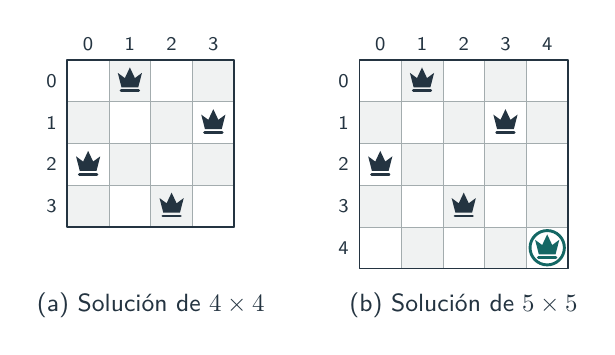
\begin{tikzpicture}[tablero A]
 \begin{scope}
  \cuadriculaA{4}\trazarRejillaA{4}
  \reinaA{0}{1}\reinaA{1}{3}\reinaA{2}{0}\reinaA{3}{2}
  \panelA{2,5.34}{(a) Solución de $4\times4$}
 \end{scope}
 \begin{scope}[shift={(7,0)}]
  \cuadriculaA{5}\trazarRejillaA{5}
  \reinaA{0}{1}\reinaA{1}{3}\reinaA{2}{0}\reinaA{3}{2}
  \aroA{4}{4}\reinaA[colorAro]{4}{4}
  \panelA{2.5,5.34}{(b) Solución de $5\times5$}
 \end{scope}
\end{tikzpicture}
\caption{Dos soluciones pequeñas. Cada corona representa una reina; el aro señala la reina
$(4,4)$, que se usa en los ejemplos siguientes.}
\label{fig:ejemplos}
\end{figure}


En todo el artículo fijamos el tamaño del tablero y agrupamos las colocaciones según
el número de reinas que faltan: éste es el sentido de \emph{capa} en el título. Por
ejemplo, si en la Figura~\ref{fig:ejemplos}(b) retiramos la reina $(4,4)$, obtenemos
una colocación de la capa $h=1$ de $5\times5$; al colocarla de nuevo pasamos a la
capa $h=0$.

La misma pregunta tiene sentido cuando faltan $h$ reinas; diremos entonces que la
colocación tiene $h$ \emph{huecos}. Llamamos \emph{capa $h$}
al conjunto $\Om_h(n)$ de colocaciones legales de $n-h$ reinas. Sean
$N_h(n)=|\Om_h(n)|$ y $\mu_h$ la ley uniforme en esa capa cuando contiene al menos
una colocación. Tomamos una colocación con ley $\mu_h$. Sus $h$ filas vacías y sus
$h$ columnas vacías se cortan en $h^2$ \emph{cruces vacíos}; cuando hablemos de la posición de los
huecos nos referiremos a la de estos cruces. Elegimos uno de ellos
uniformemente. Diremos que
está \emph{disponible} si podemos añadir allí una reina, lo que equivale a que sus dos
diagonales estén libres. Para $h>1$, este experimento pregunta por la siguiente
inserción, aunque todavía queden reinas por colocar.

La probabilidad de una inserción legal se puede expresar mediante los tamaños de dos
capas consecutivas. Cada colocación de la capa $h-1$ tiene $n-h+1$ reinas que
podemos retirar para volver a la capa $h$. A la inversa, cada colocación de la
capa $h$ ofrece $h^2$ cruces para intentar la inserción. Al contar las inserciones
legales en ambos sentidos (Lema~\ref{lem:interpretacion}) se ve que la fracción media de
cruces disponibles bajo $\mu_h$ es el cociente
\begin{equation}\label{eq:fh}
 f_h(n)=\frac{(n-h+1)\,N_{h-1}(n)}{h^2\,N_h(n)} ,
\end{equation}
que tomamos como definición de $f_h(n)$ para $1\le h\le n$. Así, $f_1(n)$ responde
exactamente a la pregunta sobre la última reina. Demostramos que, para cada $h$ fijo,
$f_h(n)$ tiende a una misma constante positiva cuando crece el tablero.

Para ver qué se promedia, volvamos a la Figura~\ref{fig:ejemplos}(b) y
retiremos las reinas $(1,3)$ y $(4,4)$. Al quedar tres reinas en $5\times5$
tenemos dos huecos y cuatro cruces (Figura~\ref{fig:cruces-vacios}). Las filas
vacías son $1$ y $4$ y las columnas vacías son $3$ y $4$. La reina de $(3,2)$
ataca $(1,4)$ por la antidiagonal de suma $5$, y $(4,3)$ por la diagonal de
diferencia $1$. Los otros dos cruces admiten una reina.

\begin{figure}[htbp]
\centering
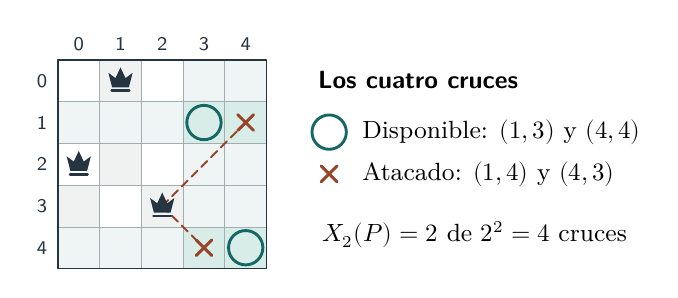
\begin{tikzpicture}[tablero A]
 \cuadriculaA{5}
 \foreach \rA in {1,4}{\fill[colorAro!7] (0,\rA) rectangle ++(5,1);}
 \foreach \cA in {3,4}{\fill[colorAro!7] (\cA,0) rectangle ++(1,5);}
 \foreach \rA in {1,4}{\foreach \cA in {3,4}{\fill[colorFondo] (\cA,\rA) rectangle ++(1,1);}}
 \trazarRejillaA{5}
 \ataqueA{3}{2}{1}{4}\ataqueA{3}{2}{4}{3}
 \reinaA{0}{1}\reinaA{2}{0}\reinaA{3}{2}
 \aroA{1}{3}\aroA{4}{4}\aspaA{1}{4}\aspaA{4}{3}
 \begin{scope}[shift={(6.0,.23)}]
  \node[anchor=west,font=\small\sffamily\bfseries] at (0,.25) {Los cuatro cruces};
  \aroA{1}{0}
  \node[anchor=west,font=\small] at (1.06,1.5) {Disponible: $(1,3)$ y $(4,4)$};
  \aspaA{2}{0}
  \node[anchor=west,font=\small] at (1.06,2.5) {Atacado: $(1,4)$ y $(4,3)$};
  \node[anchor=west,font=\small] at (.1,3.95) {$X_2(P)=2$ de $2^2=4$ cruces};
 \end{scope}
\end{tikzpicture}
\caption{Una colocación de la capa $\Omega_2(5)$. Los círculos y las aspas
ocupan las cuatro intersecciones de las filas y columnas vacías. Las líneas
discontinuas muestran por qué dos de ellas quedan bajo ataque.}
\label{fig:cruces-vacios}
\end{figure}


Escribimos $X_h(P)$ para el número de cruces disponibles en una colocación $P$.
En el ejemplo $X_2(P)=2$, de modo que un cruce elegido al azar en este tablero
admite una reina con probabilidad $2/4$. Para obtener $f_2(5)$ hay que promediar
esa fracción sobre todas las colocaciones legales de tres reinas en $5\times5$.

\subsection{Resultados principales}

Para identificar la constante, escribimos $x=h/n$ para la fracción de huecos. Al crecer $n$
con $h$ fijo, $x$ se acerca a cero. Esto lleva a estudiar el extremo de tablero lleno del perfil
variacional: la densidad $\nu_x$ en $[0,1]^2$, de masa $1-x$, que maximiza el funcional de
entropía de la Sección~\ref{subsec:variacional}. Para $x\in[0,1/2]$ tiene la forma
\[
 \nu_x(r,c)=b_x\,r_{R,x}(r)\,r_{C,x}(c)\,u_{D,x}(r-c)\,u_{A,x}(r+c),
 \qquad \int_0^1 r_{R,x}=\int_0^1 r_{C,x}=1,
\]
donde $r_{R,x}$ y $r_{C,x}$ describen los perfiles reescalados de filas y columnas
vacías, $u_{D,x}$ y $u_{A,x}$ las \emph{vacancias} de diagonales y antidiagonales (la densidad
de las que quedan vacías), y $b_x>0$ es la constante de normalización. Las propiedades del perfil se
demuestran en~\cite{Perfil}. Definimos
\begin{equation}\label{eq:F}
 F(x)=\frac{1-x}{b_x}=\int_{[0,1]^2}r_{R,x}(r)\,r_{C,x}(c)\,u_{D,x}(r-c)\,u_{A,x}(r+c)\,dr\,dc .
\end{equation}
Heurísticamente, $F(x)$ es la probabilidad de que un cruce vacío típico tenga libres sus dos
diagonales cuando hay $xn$ huecos: la posición del cruce se distribuye según $r_{R,x}r_{C,x}$ y
cada diagonal está vacía con densidad $u_{D,x}$ o $u_{A,x}$. Para las últimas capas la constante
relevante es $F(0)=1/b_0$.

\begin{teorema}[Ley de las últimas capas]\label{thm:limite}
Para cada $h\ge1$ fijo,
\[
 \lim_{n\to\infty}f_h(n)=F(0)=\frac1{b_0}\in(0,\infty).
\]
En particular, $\max_{1\le h\le K}|f_h(n)-F(0)|\to0$ para cada $K$ fijo.
\end{teorema}

Cada factor $f_j(n)$ relaciona dos capas consecutivas. Al multiplicar esas relaciones
desde $j=1$ hasta $j=h$, aparece el número de soluciones completas en el denominador.

\begin{corolario}[Cociente entre capas]\label{cor:cociente}
Para cada $h\ge1$ fijo,
\[
 \frac{N_h(n)}{Q(n)}=\frac{(n)_h}{(h!)^2\prod_{j=1}^hf_j(n)}
 \sim\frac{n^h}{(h!)^2F(0)^h},\qquad (n)_h=n(n-1)\cdots(n-h+1).
\]
\end{corolario}

El paso de la capa $h$ a la capa $h-1$ lleva la fracción de huecos de $h/n$ a
$(h-1)/n$. El corolario siguiente compara cada $f_h(n)$ con el valor de $F$
en el punto medio, $(h-\tfrac12)/n$.

\begin{corolario}[Las capas fijas no dejan constante residual]\label{cor:capas}
Para cada $K$ fijo,
\[
 \sum_{h=1}^K\log\frac{f_h(n)}{F\bigl((h-\tfrac12)/n\bigr)}\longrightarrow0,
\]
y lo mismo vale si $F((h-\tfrac12)/n)$ se sustituye por $F(h/n)$.
\end{corolario}

El número $K$ se fija antes de que crezca el tablero. Identificar el término
constante de $\log Q(n)$ exigiría controlar además las capas cuyo índice crece
con $n$. Para las dos últimas capas damos además una prueba directa de una cota inferior
explícita para $\liminf_nf_h(n)$, que no necesita la concentración de la cuenta inversa
(Sección~\ref{sec:inversa}).

\begin{teorema}[Cota inferior con constante explícita]\label{thm:positiva}
Sea $\kappa\in(0,1]$ la cota inferior de las vacancias diagonales $u_{D,x}$ y $u_{A,x}$ del perfil
(Teorema~\ref{thm:perfil}) y $a_0=(\kappa/2)^4/16$. Entonces
\[
 \liminf_{n\to\infty}f_h(n)\ge\frac{a_0}{2}>0,\qquad h=1,2.
\]
En particular, existen $c>0$ y $n_0$ tales que $f_1(n),f_2(n)\ge c$ para todo $n\ge n_0$.
\end{teorema}

El Teorema~\ref{thm:limite} ya implica la positividad de $\lim_nf_h(n)$ para cada $h$ fijo.
En efecto, \eqref{eq:F} y las cotas del Teorema~\ref{thm:perfil}(a) y~(c) dan
$F(0)\ge\kappa^2>a_0/2$. La prueba directa del Teorema~\ref{thm:positiva} está en la
Sección~\ref{sec:positiva}. Lo enunciamos sólo para las dos últimas capas porque su papel es
mostrar la cuenta directa sin la cuenta inversa de la Sección~\ref{sec:inversa}; para todo $h$
fijo, el Teorema~\ref{thm:limite} da ya una conclusión más fuerte. La constante es conservadora y el
umbral $n_0$ es existencial.

Para entender esa prueba, volvamos al caso de la última reina. Si el cruce
$(r,c)$ está atacado, la inserción en esa casilla falla. Al retirar
una reina de $(i,j)$ podemos ocupar sus \emph{destinos} $(r,j)$ e $(i,c)$ si las dos reinas nuevas son
compatibles con el resto del tablero y entre sí.
Así se aprovechan tanto la fila $r$ como la columna $c$, aunque el cruce $(r,c)$
quede sin reina.

Para cualquier $h\ge1$, llamamos \emph{reparación de un movimiento} en $(r,c)$
a esta sustitución de una reina por dos. Una reparación legal lleva la colocación
$P\in\Om_h(n)$ a la capa $h-1$. La Figura~\ref{fig:reparacion-tablero}
muestra un caso en $4\times4$. El cruce vacío $(2,1)$ está atacado por la reina
de $(3,2)$. Retiramos la reina de $(0,0)$ y colocamos dos en $(2,0)$ y $(0,1)$.
El cruce original sigue bajo ataque y queda sin ocupar. La nueva colocación ya
tiene cuatro reinas y coincide con la Figura~\ref{fig:ejemplos}(a).

\begin{figure}[htbp]
\centering
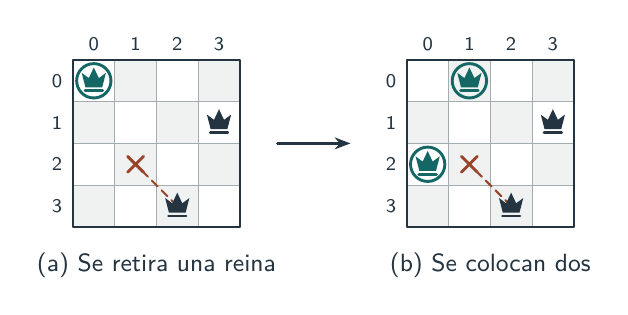
\begin{tikzpicture}[tablero A]
 \begin{scope}
  \cuadriculaA{4}\trazarRejillaA{4}
  \ataqueA{3}{2}{2}{1}\aspaA{2}{1}
  \aroA{0}{0}\reinaA[colorAro]{0}{0}\reinaA{1}{3}\reinaA{3}{2}
  \panelA{2,4.38}{(a) Se retira una reina}
 \end{scope}
 \draw[-{Stealth[length=2mm]},tintaReina,line width=.9pt] (4.9,2)--(6.65,2);
 \begin{scope}[shift={(8,0)}]
  \cuadriculaA{4}\trazarRejillaA{4}
  \ataqueA{3}{2}{2}{1}\aspaA{2}{1}
  \reinaA{1}{3}\reinaA{3}{2}
  \aroA{0}{1}\reinaA[colorAro]{0}{1}
  \aroA{2}{0}\reinaA[colorAro]{2}{0}
  \panelA{2,4.38}{(b) Se colocan dos}
 \end{scope}
\end{tikzpicture}
\caption{Una reparación legal lleva de $\Omega_1(4)$ a $\Omega_0(4)$.
Los aros identifican las piezas que cambian. El aspa marca la misma casilla
$(2,1)$ en ambos dibujos. Leyendo de derecha a izquierda se recupera la operación
inversa con el par ordenado $(2,0),(0,1)$.}
\label{fig:reparacion-tablero}
\end{figure}


Llamaremos \emph{absorbedor} de ese cruce a una reina cuya sustitución
de esta manera es legal. En la Figura~\ref{fig:reparacion-tablero}(a), sólo
sirve la de $(0,0)$. Si retiramos la de $(1,3)$, uno de sus destinos es $(1,1)$.
Si retiramos la de $(3,2)$, uno de sus destinos es $(2,2)$. En ambos casos la
reina de $(0,0)$ permanece en su sitio y ataca ese destino. Tenemos, pues, un
cruce con cero inserciones directas y una reparación legal.

Sea $A^{rc}(P)$ el número de
reparaciones legales en $(r,c)$ y $d_{h,1}(P)=\sum A^{rc}(P)$, sumando sobre los $h^2$ cruces
vacíos; el subíndice $1$ alude a las reparaciones de un movimiento, en las que se retira una sola reina.
Escribimos $\bar r=(r+\frac12)/n$ y $\bar c=(c+\frac12)/n$ para los centros de las
casillas. Para expresar cómo varía el número de reparaciones con la posición del
cruce, usamos el perfil lleno. Denotamos su densidad por $\nu_1$: el subíndice
es la masa de reinas, igual a uno, que corresponde a $x=0$. Escribimos sus factores sin
el subíndice $x$ (la constante conserva el suyo, $b_0$) y ponemos
\begin{gather*}
 \nu_1=b_0\,r_R\,r_C\,u_D\,u_A,\qquad \psi(r,c)=u_D(r-c)\,u_A(r+c),\\
 a(r,c)=\int_{[0,1]^2}\nu_1(i,j)\,\psi(r,j)\,\psi(i,c)\,di\,dj .
\end{gather*}
Se tiene $\kappa^4\le a\le1$.

\begin{teorema}[Estructura típica]\label{thm:estructura}
Sea $h\ge1$ fijo y $P$ distribuida según $\mu_h$. Los factores $r_R,r_C$, la constante $b_0$ y
las funciones $\psi$ y $a$ son los del perfil lleno del Teorema~\ref{thm:perfil}, tomado
de~\cite{Perfil}.
\begin{enumerate}[(a)]
\item \emph{Reparaciones de un movimiento.} En probabilidad,
\[
 \max_{(r,c)\ \text{cruce vacío de }P}\ \Bigl|\frac{A^{rc}(P)}{n}-a(\bar r,\bar c)\Bigr|\longrightarrow0 .
\]
\item \emph{Posición media de los huecos.} Para toda función continua $\varphi$ en $[0,1]^2$,
\[
 \E_{\mu_h}\Bigl[\frac1{h^2}\sum_{(r,c)\ \text{cruce vacío}}\varphi(\bar r,\bar c)\Bigr]
 \longrightarrow\int_{[0,1]^2}\varphi(r,c)\,r_R(r)\,r_C(c)\,dr\,dc .
\]
Para $h=1$ esto es la convergencia débil de la ley de la posición del único cruce vacío.
\item \emph{Contador sin peso.} $\E_{\mu_h}[d_{h,1}]/(h^2n)\to B_1/b_0$, donde
$B_1=\int_{[0,1]^2}\psi$.
\end{enumerate}
\end{teorema}

\begin{observacion}[Alcance]\label{obs:alcance}
\begin{enumerate}[(i)]
\item Todos los enunciados son para $h$ y $K$ fijos cuando $n\to\infty$. No se obtienen tasas de
convergencia ni uniformidad para $K=K(n)\to\infty$, y no se determina la asintótica completa
de $Q(n)$.
\item En (b), para $h>1$ sólo se identifica la medida media de los cruces vacíos: no se afirma
que las filas y las columnas vacías sean asintóticamente independientes, ni que la medida empírica
de los cruces vacíos se concentre. En (c) se trata de
convergencia de medias: por (a), $d_{h,1}/n-\sum a(\bar r,\bar c)\to0$, y el segundo término
puede seguir siendo aleatorio, de modo que no se afirma concentración de $d_{h,1}/n$.
\item El valor $F(0)\approx0{,}0809$ procede de una resolución numérica determinista del
problema variacional~\cite[Sección~9]{Perfil}, sin certificación de error. A tamaño finito los valores
exactos, obtenidos por
enumeración exhaustiva, quedan lejos del límite (por ejemplo $f_1(15)\approx0{,}114$ y
$f_2(15)\approx0{,}153$;
Tabla~\ref{tab:ilustracion}); el teorema no da información sobre la velocidad de convergencia.
\item Los Teoremas~\ref{thm:limite}, \ref{thm:positiva} y~\ref{thm:estructura} usan el perfil del
Teorema~\ref{thm:perfil}, cuyas propiedades se toman de~\cite{Perfil}; el
Apéndice~\ref{app:perfil} resume las pruebas de las cotas y de la regularidad Lipschitz.
\end{enumerate}
\end{observacion}

\subsection{Idea de la demostración}\label{subsec:idea}

La Figura~\ref{fig:esquema} resume la estructura de la prueba.

Una misma colocación puede admitir varias reparaciones en un cruce. Contamos cada
operación legal una vez desde su colocación inicial y otra desde la final. En
la segunda descripción, partimos de $P'\in\Om_{h-1}$, elegimos el par ordenado
de reinas $(r,j),(i,c)$ y las sustituimos por $(i,j)$ para recuperar $P\in\Om_h$.
Asignamos al cruce $(r,c)$ el mismo peso $w(r,c)$ en ambas descripciones. La
doble cuenta de la Sección~\ref{sec:doblecuenta} da
\[
 N_h\,\E_{\mu_h}D_w=N_{h-1}\,\E_{\mu_{h-1}}I_w,\qquad\text{luego}\qquad
 f_h=\frac{n-h+1}{n}\,\frac{\E_{\mu_h}[D_w/(h^2n)]}{\E_{\mu_{h-1}}[I_w/n^2]},
\]
donde $D_w$ e $I_w$ son los contadores directo e inverso ponderados. Para usar el
cociente elegiremos un peso para el que el denominador tenga límite positivo.

Las dos medias se toman bajo leyes distintas: $\mu_h$ en la cuenta directa y
$\mu_{h-1}$ en la inversa. Para tratar ambas, la Sección~\ref{sec:referencia}
construye un proceso aleatorio para cada capa $h$. Coloca sucesivamente piezas reales
(reinas) y piezas virtuales, que no colocan ninguna reina pero desactivan las líneas que tocan,
hasta que no queda ninguna línea activa; los pesos proceden del perfil variacional. Denotemos por
$\nu'_h$ la ley de la colocación final en la capa $h$, condicionada al éxito del proceso. Una identidad
entrópica, las estimaciones
de los normalizadores (las sumas de pesos que normalizan cada elección) y la cota inferior de
primer orden de Simkin dan
$\KL{\mu_h}{\nu'_h}=o(n)$. En consecuencia, un evento con probabilidad a lo sumo
$e^{-cn}$ bajo $\nu'_h$, con $c>0$ fijo, tiene probabilidad $o(1)$ bajo $\mu_h$.


La comparación reduce el problema a controlar las reparaciones a lo largo del
proceso. Mientras quede una fracción fija de piezas, los grados y los normalizadores
se concentran alrededor de sus trayectorias deterministas (Sección~\ref{sec:regularidad}).
Un \emph{patrón} fija qué se exige a las casillas cuya reina se retira, en una reparación o
en su operación inversa, y a las diagonales de las casillas que se ocupan: que cada casilla
tenga ya su reina o siga disponible, y que cada diagonal esté libre de toda pieza o, al
menos, de reinas. Para la cuenta directa seguimos $32$ patrones
por cada casilla candidata de un cruce, y para la inversa $16$ por cada par de casillas.
En cada familia, el cambio esperado de un patrón se expresa mediante los patrones de la
misma familia, con un error que se acota en la prueba. Resolviendo hacia atrás el sistema
lineal correspondiente se obtiene una combinación lineal de patrones, el \emph{compensador},
que coincide con el contador en el instante elegido y cuya deriva es pequeña; una
desigualdad de martingalas da entonces la concentración hasta un corte
temprano, cuando quedan unas $\delta n$ reinas por colocar. Después del corte, cada reina
cambia el contador directo de cada cruce en a lo sumo cinco unidades y el contador
inverso en $O(n)$. Al dividir por $n$ y por $n^2$, respectivamente, el efecto
de todo el tramo final es $O(\delta)$.

Una vez controlada la pérdida tras el corte, la desigualdad de entropía binaria
transfiere la concentración a la ley uniforme de cada capa. Para la cota inferior
basta la cuenta directa, pues con probabilidad tendiente a uno cada cruce vacío
admite al menos $a_0n/2$ reparaciones. Para hallar el límite hay que tener en
cuenta la posición del cruce. En $(r,c)$, la cuenta directa se concentra alrededor
de $n\,a(\bar r,\bar c)$. Al elegir el peso $w=1/a$ obtenemos
$D_{1/a}/(h^2n)\to1$. La media del contador inverso dividido por $n^2$, con ese mismo
peso, tiende a $\int\Gamma/a$,
donde $\Gamma(r,c)$ es la densidad límite de las operaciones inversas que crean el cruce $(r,c)$
(Lema~\ref{lem:nucleo}), y la identidad $\Gamma=b_0\,r_Rr_C\,a$, consecuencia de la forma producto del
perfil, da $\int\Gamma/a=b_0$. Por tanto $f_h\to1/b_0=F(0)$.
\ifverificacionLean
La Sección~\ref{sec:verificacion} describe la formalización en Lean de los enunciados
principales y precisa qué comprueba.
\fi

\begin{figure}[t]
\centering
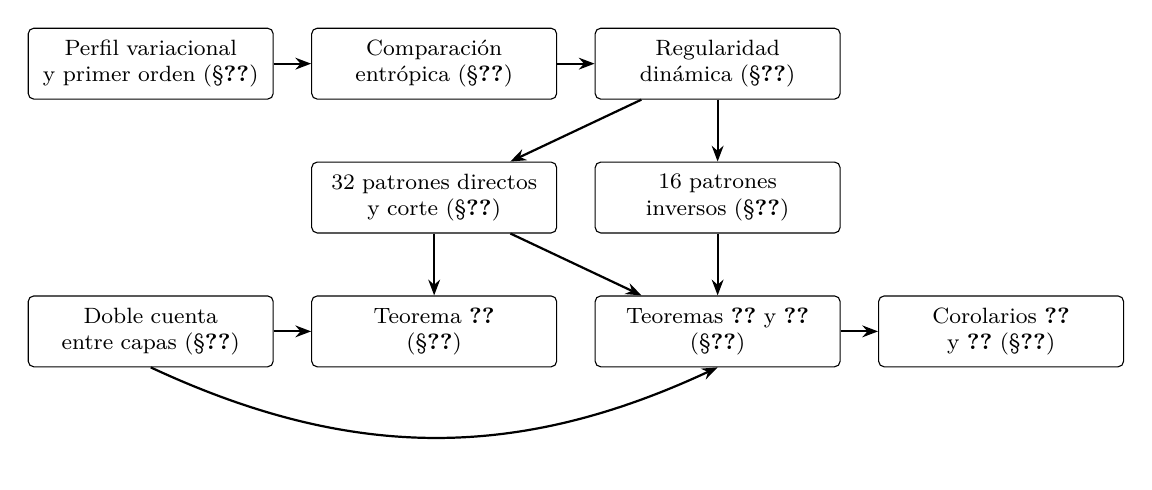
\begin{tikzpicture}[
 caja/.style={draw,rounded corners=2pt,align=center,font=\footnotesize,inner sep=3pt,
 minimum height=9mm,text width=29mm},
 flecha/.style={-{Stealth[length=2mm]},thick}]
\node[caja] (perfil) at (0,0) {Perfil variacional\\ y primer orden (§\ref{sec:preliminares})};
\node[caja] (ref) at (3.6,0) {Comparación\\ entrópica (§\ref{sec:referencia})};
\node[caja] (din) at (7.2,0) {Regularidad\\ dinámica (§\ref{sec:regularidad})};
\node[caja] (abs) at (3.6,-1.7) {32 patrones directos\\ y corte (§\ref{sec:absorbedores})};
\node[caja] (inv) at (7.2,-1.7) {16 patrones\\ inversos (§\ref{sec:inversa})};
\node[caja] (dc) at (0,-3.4) {Doble cuenta\\ entre capas (§\ref{sec:doblecuenta})};
\node[caja] (pos) at (3.6,-3.4) {Teorema~\ref{thm:positiva}\\ (§\ref{sec:positiva})};
\node[caja] (lim) at (7.2,-3.4) {Teoremas~\ref{thm:limite} y~\ref{thm:estructura}\\ (§\ref{sec:limite})};
\node[caja] (cor) at (10.8,-3.4) {Corolarios~\ref{cor:cociente}\\ y~\ref{cor:capas} (§\ref{sec:corolarios})};
\draw[flecha] (perfil) -- (ref);
\draw[flecha] (ref) -- (din);
\draw[flecha] (din) -- (abs);
\draw[flecha] (din) -- (inv);
\draw[flecha] (abs) -- (pos);
\draw[flecha] (abs) -- (lim);
\draw[flecha] (inv) -- (lim);
\draw[flecha] (dc) -- (pos);
\draw[flecha] (dc.south) to[out=-25,in=-155] (lim.south);
\draw[flecha] (lim) -- (cor);
\end{tikzpicture}
\caption{Estructura lógica de la demostración. La doble cuenta es puramente combinatoria; la
comparación entrópica de la Sección~\ref{sec:referencia} interviene en todas las flechas que
llegan a resultados bajo $\mu_h$.}
\label{fig:esquema}
\end{figure}

\subsection{Relación con trabajos previos}

Simkin~\cite{Simkin} caracteriza el término exponencial de $Q(n)$ mediante una optimización de
entropía y establece grandes desviaciones para el perfil de las soluciones completas; antes,
Luria~\cite{Luria} había obtenido cotas superiores con el método de entropía. La cota inferior
de primer orden que usamos procede del resultado de Simkin (Teorema~\ref{thm:simkin}). Para
probarla, Simkin fija una \emph{queenon} escalonada, es decir, una queenon
(Sección~\ref{sec:preliminares}) de densidad constante en cada bloque de una cuadrícula; en cada
paso elige un bloque con la probabilidad que esa medida le asigna, coloca en él una
reina al azar entre las casillas disponibles y, al final, completa la colocación con
absorbedores~\cite[Sección~5]{Simkin}. Luria y Simkin~\cite{LS} construyen casi-soluciones
mediante un proceso voraz aleatorio y las completan con absorbedores para obtener una cota
inferior de conteo, y Bowtell y Keevash~\cite{BK} estudian el conteo toroidal y sus
consecuencias para el tablero ordinario. El proceso de referencia y los absorbedores de este
trabajo siguen ese espíritu, pero el éxito bajo un proceso de construcción no identifica por sí
solo la ley uniforme sobre las colocaciones con $h$ huecos: esa identificación es el papel de
la comparación entrópica. Comparar la ley uniforme con la del resultado de un proceso aleatorio
es la herramienta principal del trabajo de Kwan~\cite{Kwan} sobre sistemas triples de Steiner.
A su vez, la doble cuenta de reparaciones entre capas consecutivas es una forma del método de
conmutaciones (\emph{switchings})~\cite{McKayWormald,HMcK}.

Completar una colocación parcial dada es un problema que se remonta a 1850 y es
NP-completo~\cite{GJN}. Glock, Munhá Correia y
Sudakov~\cite{GMS} prueban que toda colocación legal de a lo sumo $n/60$ reinas puede
completarse y construyen colocaciones no completables de tamaño cercano a $n/4$;
Nielsen~\cite{Nielsen} mejora la cota superior del umbral extremal a $0{,}216\,n$ para $n$
suficientemente grande. Esos
enunciados son de peor caso; aquí se estudian probabilidades bajo la ley uniforme de
colocaciones casi completas.

Hasta donde sabemos, los
Teoremas~\ref{thm:limite} y~\ref{thm:estructura} y el Corolario~\ref{cor:cociente} son nuevos.
No se reclama novedad para las herramientas generales: regla de la cadena de la entropía
relativa, comparación con procesos aleatorios~\cite{Kwan}, dobles cuentas y
conmutaciones~\cite{HMcK}, método de ecuaciones diferenciales~\cite{Wormald} y desigualdades de
concentración~\cite{AlonSpencer}.

\section{Preliminares}\label{sec:preliminares}

\subsection{Notación}

Indexamos filas y columnas por $\{0,\dots,n-1\}$. La casilla $(r,c)$ está en la fila $r$, la
columna $c$, la diagonal $r-c\in\{-(n-1),\dots,n-1\}$ y la antidiagonal
$r+c\in\{0,\dots,2n-2\}$. Llamamos \emph{líneas} a filas, columnas, diagonales y antidiagonales,
y $R,C,D,A$ a sus cuatro familias, con $n$, $n$, $2n-1$ y $2n-1$ elementos. El tablero es así un
hipergrafo $4$-partito y $4$-uniforme cuyos vértices son las líneas y cuyas aristas son las
casillas, cada una con sus cuatro líneas. Dos líneas distintas están juntas en a lo sumo una
casilla (\emph{codegrado uno}). Una colocación legal es un emparejamiento de este hipergrafo.

Para $P\in\Om_h(n)$, $R_\vac(P)$ y $C_\vac(P)$ son las $h$ filas y las $h$ columnas vacías, y
$X_h(P)$ es el número de cruces vacíos disponibles. Para coordenadas continuas usamos los centros
$\bar r=(r+\frac12)/n$, $\bar c=(c+\frac12)/n$; una diagonal o antidiagonal recibe la coordenada
que inducen los centros de sus casillas, $\bar r-\bar c\in[-1,1]$ o $\bar r+\bar c\in[0,2]$.

Salvo indicación, $n\to\infty$ con $h$ (o $K$) fijo; $c,C$ denotan constantes positivas que
pueden cambiar de una aparición a otra y cuya dependencia de parámetros fijos se indica con
subíndices. Para leyes $\mu,\nu$ en un conjunto finito,
$\KL{\mu}{\nu}=\sum\mu\log(\mu/\nu)$ es la entropía relativa (infinita si
$\mu\not\ll\nu$). Usaremos que es no negativa y que no aumenta al aplicar una misma función a
ambas leyes (procesamiento de datos)~\cite{CoverThomas}.

\subsection{Interpretación de \texorpdfstring{$f_h$}{fh}}

En la Figura~\ref{fig:cruces-vacios} contamos los cruces en una colocación
particular. Al sumar el mismo contador sobre toda la capa obtenemos la
identidad siguiente.

\begin{lema}\label{lem:interpretacion}
Para $1\le h\le n$, $\E_{\mu_h}[X_h]=h^2f_h(n)$. En particular, $f_1(n)$ es la probabilidad de
que una colocación uniforme de $\Om_1(n)$ pueda completarse a una solución.
\end{lema}

\begin{proof}
Contamos los pares $(P,P')$ con $P\in\Om_h$, $P'\in\Om_{h-1}$ y $P\subset P'$. Cada $P'$ tiene
$n-h+1$ reinas y al retirar cualquiera de ellas se obtiene un $P$ distinto: hay
$(n-h+1)N_{h-1}$ pares. Recíprocamente, añadir una reina a $P$ da una colocación legal si y
sólo si la reina ocupa un cruce vacío disponible: hay $X_h(P)$ extensiones. Así
$N_h\E_{\mu_h}X_h=(n-h+1)N_{h-1}$, que es la identidad buscada. Si $h=1$, $X_1\in\{0,1\}$ y
$X_1(P)=1$ exactamente cuando $P$ se completa.
\end{proof}

\subsection{El problema variacional y el perfil}\label{subsec:variacional}

La doble cuenta anterior es exacta para cada tamaño. Para estudiar su límite
necesitamos una descripción del tablero que conserve las restricciones de fila,
columna y diagonales al pasar a coordenadas continuas.

Para una masa $\rho\in(0,1]$, una densidad \emph{admisible} es una función medible
$\nu\ge0$ en $[0,1]^2$ con $\int\nu=\rho$ cuyas proyecciones (o marginales) sobre las cuatro familias,
\[
 m_R(r)=\int_0^1\nu(r,c)\,dc,\quad m_C(c)=\int_0^1\nu(r,c)\,dr,\quad
 m_D(d)=\int_{r-c=d}\nu,\quad m_A(s)=\int_{r+c=s}\nu,
\]
no exceden uno (las dos últimas integran a lo largo de la fibra, parametrizada por $r$). Sus
vacancias son $u_f=1-m_f$ en $I_R=I_C=[0,1]$, $I_D=[-1,1]$, $I_A=[0,2]$; así
$\int u_R=\int u_C=1-\rho$ y $\int u_D=\int u_A=2-\rho$. El funcional de entropía es
\[
 s[\nu]=-3\rho-\int\nu\log\nu-\sum_{f\in\{R,C,D,A\}}\int_{I_f}u_f\log u_f ,
\]
y $s^*(\rho)$ es su supremo sobre las densidades admisibles de masa $\rho$; ponemos
$s_1=s^*(1)$. Para $0<\rho<1$ el óptimo $\nu$ es positivo y satisface la ecuación de Euler
$\nu=\lambda_\rho\,u_Ru_Cu_Du_A$, con una constante $\lambda_\rho>0$, la \emph{actividad}~\cite[Teorema~3.1 y Lema~3.3]{Perfil}.

Con $x=1-\rho$ se reescala: $r_R=u_R/x$, $r_C=u_C/x$ y $b_x=\lambda_\rho x^2$, la actividad reescalada. Entonces
\begin{equation}\label{eq:perfil}
 \nu=b_x\,r_Rr_Cu_Du_A,\qquad \int r_R=\int r_C=1,
\end{equation}
y las ecuaciones de Euler se escriben
\begin{equation}\label{eq:euler}
 r_R=\frac1{x+b_xJ_R},\quad r_C=\frac1{x+b_xJ_C},\quad
 u_D=\frac1{1+b_xJ_D},\quad u_A=\frac1{1+b_xJ_A},
\end{equation}
donde cada $J_f$ integra a lo largo de la fibra de $f$ el producto de los otros tres factores;
por ejemplo $J_R(r)=\int_0^1r_C(c)u_D(r-c)u_A(r+c)\,dc$. En efecto, la masa de la fila $r$ es
$1-xr_R(r)=b_xr_R(r)J_R(r)$. Integrando~\eqref{eq:perfil} se obtiene la expresión~\eqref{eq:F}
de $F(x)=(1-x)/b_x$. Escribimos $\nu_x$ y $(b_x,r_{R,x},r_{C,x},u_{D,x},u_{A,x})$ cuando haga
falta indicar $x$; el subíndice es entonces la fracción de huecos, no la masa
(en~\cite{Perfil} las densidades se indexan por la masa: nuestra $\nu_x$ es allí $\nu_{1-x}$). La única
excepción es la densidad de masa uno, que corresponde a $x=0$ y se denota $\nu_1$, como
en~\cite{Perfil}.

\begin{teorema}[El perfil cerca del tablero lleno~\cite{Perfil}]\label{thm:perfil}
Existen constantes $0<\kappa\le1$, $0<\underline r\le M<\infty$, $0<b_-\le b_+<\infty$ y
$L_*<\infty$ tales que, para todo $x\in(0,1/2]$, el perfil óptimo de masa $1-x$~\cite[Teorema~3.1]{Perfil}, reescalado como
en~\eqref{eq:perfil}, satisface~\eqref{eq:euler} y:
\begin{enumerate}[(a)]
\item $b_-\le b_x\le b_+$, $\ \underline r\le r_{R,x},r_{C,x}\le M$ y
$\kappa\le u_{D,x},u_{A,x}\le1$;
\item $r_{R,x},r_{C,x},u_{D,x},u_{A,x}$ son Lipschitz en sus intervalos con constante a lo sumo
$L_*$, y $\nu_x$ es acotada y Lipschitz, uniformemente en $x$;
\item cuando $x\downarrow0$ convergen uniformemente a límites $(b_0,r_R,r_C,u_D,u_A)$ que
satisfacen~\eqref{eq:euler} con $x=0$ y las mismas cotas.
\end{enumerate}
En particular, $\nu_1=b_0r_Rr_Cu_Du_A$ es una densidad continua en $[0,1]^2$, de masa uno, con
marginales de filas y columnas iguales a uno y vacancias diagonales $u_D=1-m_D$ y $u_A=1-m_A$, de
modo que $\int u_D=\int u_A=1$; $\nu_1$ es el único maximizador de $s$ entre las densidades
admisibles de masa uno, así que $s[\nu_1]=s^*(1)=s_1$; y $F$ es continua en $0$ con
$F(0)=1/b_0>0$.
\end{teorema}

Las afirmaciones (a) y (c) son las Proposiciones~4.2, 5.2 y~5.3 de~\cite{Perfil}; que el
límite $\nu_1$ sea el único maximizador de masa uno es su Proposición~5.1 junto con la~5.2; la
regularidad Lipschitz uniforme (b) es su Teorema~7.7, y la continuidad de $F$ en $0$, con
$F(0)=1/b_0$, es su Teorema~8.1. El Apéndice~\ref{app:perfil} resume esas pruebas y da valores
explícitos de las constantes. No se usa ninguna identificación del perfil con leyes discretas de colocaciones:
el Teorema~\ref{thm:perfil} es un enunciado sobre el problema continuo.

\subsection{El primer orden de Simkin}

\begin{teorema}[{\cite[Teorema~2.11]{Simkin}}]\label{thm:simkin}
$\log Q(n)\ge n\log n+ns_1-o(n)$, con $s_1=s^*(1)=s[\nu_1]$.
\end{teorema}

El Teorema~2.11 de~\cite{Simkin} se enuncia para las
\emph{queenons}~\cite[Definiciones~2.1, 2.3 y~2.4]{Simkin}, que forman el cierre débil de los
permutones escalonados con marginales diagonales subuniformes. Tras trasladar el cuadrado a
$[-\frac12,\frac12]^2$, una densidad con marginales de filas y columnas iguales a uno es un
permutón, y tener marginales diagonales subuniformes equivale a $m_D,m_A\le1$.

\begin{lema}\label{lem:queenon}
La medida de densidad $\nu_1$, trasladada a $[-\frac12,\frac12]^2$, es una queenon.
\end{lema}

\begin{proof}
Por el Teorema~\ref{thm:perfil}, $\nu_1$ es continua en el cuadrado cerrado, tiene marginales
de filas y columnas iguales a uno, y sus proyecciones diagonales cumplen
$m_D=1-u_D\le1-\kappa$ y $m_A=1-u_A\le1-\kappa$. Para $N\ge1$, sea $\nu^{(N)}$ la densidad que
en cada casilla de la cuadrícula $N\times N$ vale el promedio de $\nu_1$ en esa casilla. En una
franja de filas de anchura $1/N$, la marginal de filas de $\nu^{(N)}$ es el promedio de la de
$\nu_1$, que vale uno; lo mismo ocurre con las columnas, así que $\nu^{(N)}$ es un permutón
escalonado. Si $\omega$ es el módulo de continuidad uniforme de $\nu_1$, entonces
$|\nu^{(N)}-\nu_1|\le\omega(\sqrt2/N)$ y, como las fibras diagonales tienen longitud
paramétrica (en $r$) a lo sumo uno, $m_D[\nu^{(N)}],m_A[\nu^{(N)}]\le1-\kappa+\omega(\sqrt2/N)\le1$
para $N$ grande. Ésa es la normalización de~\cite{Simkin}: la imagen de la medida por
$(r,c)\mapsto r\mp c$ tiene por densidad la integral de fibra en $r$, porque el jacobiano es uno.
Así $\nu^{(N)}$ tiene marginales diagonales subuniformes y converge uniformemente a $\nu_1$,
luego en variación total y, en particular, débilmente.
\end{proof}

Por el Lema~\ref{lem:queenon}, el Teorema~2.11 de~\cite{Simkin} se aplica a $\nu_1$ tal como
está enunciado; no hace falta su Observación~2.7, que lo extiende a todos los permutones con
marginales diagonales subuniformes. Tras la traslación, las densidades de vacancia diagonal son $u_D,u_A$, ambas de integral
uno; en la Definición~2.9 de~\cite{Simkin}, cada divergencia respecto de la uniforme en $[-1,1]$
vale $\int u\log u+\log2$, y las dos constantes se cancelan con $2\log2$. El funcional de
Simkin en $\nu_1$ es, por tanto,
$-3-\int\nu_1\log\nu_1-\int u_D\log u_D-\int u_A\log u_A=s[\nu_1]=s_1$. La cota inferior de
su Teorema~2.11 para este perfil da el enunciado: primero se fija la tolerancia, se toma el
límite inferior en $n$ y después se hace tender la tolerancia a cero. No se obtiene de ahí
ninguna tasa para el resto, y escribimos
\begin{equation}\label{eq:Delta}
 \Delta_n=\bigl[n\log n+ns_1-\log Q(n)\bigr]_+=o(n).
\end{equation}

\subsection{El valor variacional cerca del tablero lleno}

\begin{lema}\label{lem:borde}
Cuando $x\downarrow0$, $s^*(1-x)-s^*(1)=2x\log(1/x)+O(x)$. En consecuencia, para $K$ fijo y
$0\le h\le K$,
\[
 n\bigl[s^*(1-h/n)-s_1\bigr]=2h\log n+O_K(1).
\]
\end{lema}

Es la Proposición~8.3 de~\cite{Perfil}, donde también se prueban la desigualdad de soporte
(Teorema~3.1(d), donde $\theta=-\log\lambda_\rho$) y la continuidad de $s^*$ en $\rho=1$ (Proposición~5.1). Incluimos la prueba
por completitud.

\begin{proof}
El funcional $s$ es cóncavo en el dominio admisible. En un perfil positivo
$\nu=\lambda_\rho\prod_fu_f$, su derivada en la dirección de una variación admisible $\dot\nu$,
con $\int\dot\nu=\dot\rho$, es
\[
 \dot s=\int\Bigl[-3-1-\log\nu+\sum_f(1+\log u_f)\Bigr]\dot\nu=-\log\lambda_\rho\;\dot\rho ,
\]
pues $-\log\nu+\sum_f\log u_f=-\log\lambda_\rho$ y $-3-1+4=0$. La concavidad y la
estacionariedad a masa fija identifican el valor $s^*(\rho)$ y dan la desigualdad de soporte
\[
 s^*(\rho')\le s^*(\rho)-\log\lambda_\rho\,(\rho'-\rho).
\]
En compactos de $(0,1)$, $s^*$ es cóncava y por tanto absolutamente continua, y en sus puntos de
derivabilidad el supergradiente $-\log\lambda_\rho$ es su derivada. Las cotas bilaterales de
$b_x=\lambda_\rho(1-\rho)^2$ dan $-\log\lambda_\rho=2\log(1-\rho)+O(1)$. Por el
Teorema~\ref{thm:perfil}(c) y la continuidad de $u\log u$, el valor óptimo de masa $1-x$ tiende a
$s[\nu_1]$, que es $s^*(1)$ porque $\nu_1$ es el maximizador de masa uno
(Teorema~\ref{thm:perfil}); ésta es la continuidad de $s^*$ en $\rho=1$. Junto con la
integrabilidad de $\log(1-\rho)$, permite integrar:
\[
 s^*(1)-s^*(1-x)=\int_{1-x}^1\bigl[2\log(1-\rho)+O(1)\bigr]d\rho=2x\log x-2x+O(x).
\]
Esto es la primera afirmación. La segunda se obtiene con $x=h/n$:
$n[2(h/n)\log(n/h)+O(h/n)]=2h\log n+O_K(1)$.
\end{proof}

No se ha diferenciado el perfil respecto de su parámetro: sólo se usa la concavidad.

\subsection{Dos lemas de entropía relativa}

\begin{lema}[Condicionar al éxito]\label{lem:exito}
Sean $\PP,\QQ$ leyes en un conjunto finito y $S$ un evento con $\PP(S)=1$ y $\QQ(S)>0$.
Entonces $\KL{\PP}{\QQ(\cdot\mid S)}=\KL{\PP}{\QQ}+\log\QQ(S)$. En particular,
$\QQ(S)\ge e^{-\KL{\PP}{\QQ}}$ y $\KL{\PP}{\QQ(\cdot\mid S)}\le\KL{\PP}{\QQ}$.
\end{lema}

\begin{proof}
En $S$, $\QQ(\omega\mid S)=\QQ(\omega)/\QQ(S)$; se toma la esperanza de
$\log(\PP/\QQ(\cdot\mid S))=\log(\PP/\QQ)+\log\QQ(S)$ bajo $\PP$. La no negatividad del primer
miembro da las dos consecuencias.
\end{proof}

\begin{lema}[Transferencia binaria]\label{lem:binaria}
Sean $\mu,\nu$ leyes en un conjunto finito y $B$ un evento con $\nu(B)<1$. Entonces
\[
 \mu(B)\log\frac1{\nu(B)}\le\KL{\mu}{\nu}+\log2 .
\]
Si $\nu(B)=0$ y $\KL{\mu}{\nu}<\infty$, entonces $\mu(B)=0$.
\end{lema}

\begin{proof}
Sean $p=\mu(B)$ y $p'=\nu(B)$. Por procesamiento de datos aplicado al indicador de $B$,
\[
\begin{aligned}
 \KL{\mu}{\nu}&\ge p\log\frac p{p'}+(1-p)\log\frac{1-p}{1-p'}\\
 &\ge p\log\frac1{p'}+p\log p+(1-p)\log(1-p)\ge p\log\frac1{p'}-\log2 .
\end{aligned}
\]
El caso $p'=0$ es la continuidad absoluta.
\end{proof}

En las Secciones~\ref{sec:regularidad}--\ref{sec:inversa} usaremos además la desigualdad de
Azuma--Hoeffding para martingalas con incrementos acotados~\cite{AlonSpencer} y la desigualdad
de Gronwall discreta, en la forma habitual del método de ecuaciones diferenciales~\cite{Wormald}.

\section{Proceso de referencia y comparación entrópica}\label{sec:referencia}

El perfil continuo proporciona los pesos para construir colocaciones paso a paso.
El objetivo de esta sección es comparar la ley de las colocaciones así construidas,
condicionada al éxito, con la ley uniforme de la capa. La cota de entropía relativa
permitirá trasladar a esta última las estimaciones obtenidas durante la construcción.

Fijamos $K$ y $0\le h\le K$, y ponemos
\[
 q=n-h,\qquad N=2n-1,\qquad H=N-q=n+h-1 .
\]
En esta sección y en las dos siguientes, para $h\ge1$ el perfil se evalúa en el parámetro
objetivo $x_*=h/n$, fijo durante todo el proceso, y omitimos el subíndice $x_*$. Donde aparezcan
a la vez este perfil objetivo y el perfil lleno, como en la Sección~\ref{subsec:trayectoria},
escribiremos de nuevo el subíndice $x_*$ en el primero. La capa $h=0$
se trata por separado en la Sección~\ref{subsec:h0}.

\subsection{Hipergrafo aumentado y pesos}

Se añaden $n-1$ vértices \emph{ficticios} a las filas y otros tantos a las columnas, de modo que
cada una de las cuatro familias tiene $N$ vértices. Las \emph{aristas reales} son las $n^2$
casillas, con sus cuatro líneas físicas. Las \emph{aristas virtuales} son todas las cuaternas
con un vértice de cada familia, físico o ficticio. El color (real o virtual) forma parte de la
arista: una arista virtual es distinta de una real aunque tengan los mismos vértices.

En la Figura~\ref{fig:cruces-vacios}, las líneas de $(3,2)$ son $R_3$, $C_2$,
$D_1$ y $A_5$, pues $3-2=1$ y $3+2=5$.
Una elección real en esa casilla coloca una reina. Una elección virtual con
esas mismas cuatro líneas las desactiva en el proceso sin colocar ninguna
reina en el tablero. Esta distinción se usará al contar las reparaciones. Llamaremos \emph{piezas} a las
aristas de una
trayectoria, es decir, a las que elige el proceso, reales o virtuales según su color.

Para $h\ge1$, los pesos de vértice son $u_R(\bar r)=x_*r_R(\bar r)$ en las filas físicas,
$u_C(\bar c)=x_*r_C(\bar c)$ en las columnas físicas, $u_D$ y $u_A$ en las coordenadas inducidas
de diagonales y antidiagonales, y $1$ en los vértices ficticios. Todos son positivos. El peso de
una arista, real o virtual, es el producto $\varpi(e)=\prod_{v\in e}u_v$; por el
Teorema~\ref{thm:perfil}(a), toda arista real tiene peso entre $cx_*^2$ y $Cx_*^2$.

\subsection{El proceso}

\begin{definicion}[Proceso de referencia]\label{def:referencia}
Se preasigna, sin revelarla, una palabra uniforme con $q$ colores reales y $H$ virtuales. En
cada paso $t=1,\dots,N$ se revela sólo el siguiente color, se elige una arista disponible (con
sus cuatro vértices todavía activos) de ese color, con probabilidad proporcional a su peso, y se
desactivan sus cuatro vértices. Una pieza virtual no coloca ninguna reina. Si el normalizador
del color pedido, es decir, la suma de los pesos de sus aristas disponibles, es cero, el proceso pasa a un
estado de fallo. $\QQ_h$ es la ley de las
trayectorias y $S$ el evento de éxito (los $N$ pasos se completan).
\end{definicion}

En $S$, las $q$ aristas reales elegidas son casillas sin líneas comunes, es decir, una
colocación de $\Om_h(n)$: la \emph{colocación final}. Sea $\nu'_h$ su ley bajo
$\QQ_h(\cdot\mid S)$. En las elecciones reales puede cancelarse el factor común $x_*^2$ sin
cambiar la ley; no se cancela en las virtuales. La referencia no necesita tener éxito con
probabilidad próxima a uno.

\subsection{La ley de comparación}

\begin{definicion}[Ley de comparación]\label{def:comparacion}
Se elige $P\in\Om_h(n)$ uniforme; después, una completación virtual uniforme, es decir, un
emparejamiento perfecto por aristas virtuales de los $H$ vértices libres de cada familia (hay
$(H!)^3$); finalmente, un orden uniforme de las $N$ piezas. $\PP_h$ es la ley de la sucesión de
aristas resultante.
\end{definicion}

Representamos el orden uniforme mediante tiempos independientes y uniformes en $[0,1]$
asociados a las piezas; las piezas se revelan en orden creciente de tiempo. (La uniformidad del
tiempo de una pieza aislada no bastaría: se usa la independencia.) Estos tiempos independientes,
junto con la desigualdad de Jensen del Lema~\ref{lem:normalizadores}(iii), son el recurso de las
cotas por entropía de Radhakrishnan~\cite{Radhakrishnan} y de Linial y Luria~\cite{LinialLuria}.
La ley $\PP_h$ proyecta
exactamente en $\mu_h$, y toda trayectoria de su soporte tiene probabilidad positiva bajo
$\QQ_h$: la siguiente pieza del emparejamiento completo sigue disponible y tiene peso positivo.
En particular $\PP_h(S)=1$.

\subsection{La identidad entrópica}

Sean $W_R(t)$ y $W_V(t)$ los pesos totales de las aristas disponibles de cada color antes del
paso $t$, y $\col(t)$ el color revelado en ese paso.

\begin{lema}\label{lem:identidad}
Para $1\le h\le K$,
\[
 \KL{\PP_h}{\QQ_h}=\E_{\PP_h}\sum_{t=1}^N\log W_{\col(t)}(t)-\sum_v\log u_v-\log N_h-\log q!
 -4\log H!,
\]
donde $\sum_v$ recorre los $4N$ vértices.
\end{lema}

\begin{proof}
Sea $\omega$ una trayectoria del soporte de $\PP_h$. Entonces $\PP_h(\omega)=[N_h(H!)^3N!]^{-1}$.
Bajo $\QQ_h$, la palabra de colores tiene probabilidad $\binom Nq^{-1}$ y cada elección tiene
probabilidad $\varpi(e_t)/W_{\col(t)}(t)$. Como el emparejamiento completo cubre cada vértice
exactamente una vez, el producto de los pesos elegidos es $\prod_vu_v$, independiente del
emparejamiento y del orden. Por tanto
\[
 \log\frac{\PP_h(\omega)}{\QQ_h(\omega)}=\sum_t\log W_{\col(t)}(t)-\sum_v\log u_v
 -\log\bigl[N_h(H!)^3N!\bigr]+\log\binom Nq ,
\]
y $-\log[(H!)^3N!]+\log\binom Nq=-\log q!-4\log H!$. Se toma la esperanza bajo $\PP_h$.
\end{proof}

\subsection{Normalizadores}

\begin{lema}\label{lem:normalizadores}
Sea $\rho=1-x_*=q/n$. Uniformemente en $1\le h\le K$:
\begin{enumerate}[(i)]
\item $W_R(0)=n^2\rho/\lambda_\rho\,(1+O(n^{-1}))\asymp x_*^2n^2$ y $W_V(0)=H^4(1+O(n^{-1}))$;
\item $\sum_v\log u_v=n\sum_f\int_{I_f}\log u_f+O(1)$;
\item $\E_{\PP_h}\sum_t\log W_{\col(t)}(t)\le q\log W_R(0)+H\log W_V(0)-4N+O(n^{2/3})$.
\end{enumerate}
\end{lema}

\begin{proof}
(i) Por cuadratura de los factores reescalados, positivos y Lipschitz,
$W_R(0)=x_*^2n^2\int r_Rr_Cu_Du_A\,(1+O(n^{-1}))=x_*^2n^2\rho/b\,(1+O(n^{-1}))$, y
$x_*^2/b=1/\lambda_\rho$. En cada familia la suma de pesos es $H+O(1)$: en filas se suman
$n-1$ ficticios y $\sum u_R=nx_*+O(x_*)$; en diagonales, $\sum u_D=n\int u_D+O(1)=n(2-\rho)+O(1)$.
Como $W_V(0)$ es el producto de las cuatro sumas, $W_V(0)=H^4(1+O(n^{-1}))$.

(ii) En filas, $\sum\log u_R=n\log x_*+\sum\log r_R(\bar r)$: la constante $\log x_*$ se suma
exactamente $n$ veces y $\log r_R$ es uniformemente Lipschitz, de modo que el error de
cuadratura es $O(1)$ sin depender de $1/x_*$. Lo mismo en columnas, diagonales y
antidiagonales; los ficticios aportan cero.

(iii) Fijemos un emparejamiento completado y una pieza $p$, revelada en el tiempo
$\mathsf t_p\in[0,1]$; sea $z=1-\mathsf t_p$ y sea $W^{(p)}$ el normalizador del color de $p$ en el
momento en que se revela. Condicionalmente al emparejamiento y a $\mathsf t_p$, cada una de las
demás piezas sigue sin revelar, independientemente, con probabilidad $z$. Una arista
\emph{ordinaria} del color de $p$ tiene sus cuatro vértices cubiertos por cuatro piezas distintas
de $p$ y está disponible con probabilidad $z^4$. Por codegrado uno hay $O(n)$ aristas reales
excepcionales, de peso $O(x_*^2)$; salvo la contenida en $p$, cada una necesita al menos otra
pieza sin revelar y está disponible con probabilidad a lo sumo $z$. Las excepciones virtuales son
$O(n^3)$, de peso a lo sumo uno. Así, uniformemente en el emparejamiento,
\[
 \E W^{(p)}\le W_R(0)z^4+Cx_*^2nz+Cx_*^2\ \ (p\text{ real}),\qquad
 \E W^{(p)}\le W_V(0)z^4+Cn^3z+C\ \ (p\text{ virtual}).
\]
Por Jensen, (i) y $\log(1+u+v)\le\log(1+u)+\log(1+v)$, los términos de error son de orden
$1/(nz^3)$ y $1/(n^2z^4)$ para reales, y $1/(nz^3)$ y $1/(n^4z^4)$ para virtuales. Como
$\int_0^1\log z^4\,dz=-4$ y, para $c>0$ fijo, $\int_0^1\log(1+cn^{-1}z^{-3})\,dz=O(n^{-1/3})$,
$\int_0^1\log(1+cn^{-2}z^{-4})\,dz=O(n^{-1/2})$ e $\int_0^1\log(1+cn^{-4}z^{-4})\,dz=O(n^{-1})$,
\[
 \E\log W^{(p)}\le\log W_{\col(p)}(0)-4+O(n^{-1/3}).
\]
Como $\sum_t\log W_{\col(t)}(t)=\sum_p\log W^{(p)}$, sumando sobre las $N$ piezas se obtiene
(iii).
\end{proof}

\begin{lema}\label{lem:retirada}
$N_h(n)\ge\binom nh Q(n)/h!$.
\end{lema}

\begin{proof}
Al retirar $h$ reinas de una solución se obtiene una colocación de $\Om_h$, y cada
colocación de $\Om_h$ tiene a lo sumo $h!$ completaciones, porque las $h$ reinas que faltan
ocupan una permutación de los $h$ cruces vacíos. Luego $\binom nhQ\le h!N_h$.
\end{proof}

\begin{teorema}[Comparación entrópica]\label{thm:comparacion}
Sea $K$ fijo. Existe $d_n=\Delta_n+C_Kn^{2/3}+O_K(\log n)=o(n)$ tal que, para todo
$0\le h\le K$,
\[
 \KL{\PP_h}{\QQ_h}\le d_n,\qquad \QQ_h(S)\ge e^{-d_n},\qquad \KL{\mu_h}{\nu'_h}\le d_n .
\]
\end{teorema}

\begin{proof}[Demostración para $1\le h\le K$]
Por los Lemas~\ref{lem:identidad} y~\ref{lem:normalizadores} y Stirling
($\log H!=H\log H-H+O(\log n)$, y lo mismo para $q!$),
\[
 \KL{\PP_h}{\QQ_h}\le q\log\frac{n^2\rho}{\lambda_\rho}-4q-n\sum_f\int\log u_f-(q\log q-q)
 -\log N_h+Cn^{2/3}+O(\log n),
\]
donde se usó $4H\log H-4\log H!=4H+O(\log n)$ y $N-H=q$. Con $q=n\rho$,
$q\log(n^2\rho)-q\log q=q\log n$, de modo que el segundo miembro es
$q\log n+n[-3\rho-\rho\log\lambda_\rho-\sum_f\int\log u_f]-\log N_h+Cn^{2/3}+O(\log n)$. La
expresión entre corchetes es $s^*(\rho)$: por la ecuación de Euler,
$\int\nu\log\nu=\rho\log\lambda_\rho+\sum_f\int m_f\log u_f$ y
$\int m_f\log u_f=\int\log u_f-\int u_f\log u_f$. Así
\[
 \KL{\PP_h}{\QQ_h}\le q\log n+ns^*(q/n)-\log N_h+Cn^{2/3}+O(\log n).
\]
Por el Lema~\ref{lem:borde}, $ns^*(q/n)=ns_1+2h\log n+O_K(1)$; por el Lema~\ref{lem:retirada},
$-\log N_h\le-\log Q-\log\binom nh+\log h!=-\log Q-h\log n+O_K(1)$. Los términos en
$\log n$ se cancelan exactamente ($-h+2h-h=0$) y, por~\eqref{eq:Delta},
$\KL{\PP_h}{\QQ_h}\le\Delta_n+C_Kn^{2/3}+O_K(\log n)=d_n$. No se usa ninguna tasa para
$\Delta_n$. Como $\PP_h(S)=1$, el Lema~\ref{lem:exito} da $\QQ_h(S)\ge e^{-d_n}$ y
$\KL{\PP_h}{\QQ_h(\cdot\mid S)}\le d_n$; al proyectar en la colocación final, el
procesamiento de datos da $\KL{\mu_h}{\nu'_h}\le d_n$.
\end{proof}

\subsection{La capa cero}\label{subsec:h0}

En $h=0$ los pesos $x_*r_R$ de filas y columnas físicas se anulan, de modo que no se puede
sustituir $x_*=0$ en la construcción anterior. Se usa una extensión límite explícita.

\begin{definicion}[Referencia en la capa cero]\label{def:referencia_cero}
Sea $q=n$, $H=n-1$, $N=2n-1$. Las aristas reales tienen peso $v_e=r_Rr_Cu_Du_A$, evaluado en el
perfil lleno. Los pesos de vértice para las aristas virtuales son cero en filas y columnas
físicas, uno en sus ficticios, y $u_D,u_A$ en diagonales y antidiagonales. La palabra de colores
sigue siendo uniforme y, si falta una arista del color pedido, el proceso pasa al estado de
fallo. Las leyes $\QQ_0$, $\PP_0$ y $\nu'_0$ se definen como antes.
\end{definicion}

\begin{proof}[Demostración del Teorema~\ref{thm:comparacion} para $h=0$]
\emph{Soporte.} Toda solución usa todas las filas y columnas físicas, así que sus completaciones
virtuales usan exclusivamente los vértices ficticios de filas y columnas. Por tanto $\PP_0$,
uniforme sobre soluciones, completaciones y órdenes, tiene soporte positivo bajo $\QQ_0$ pese a
los pesos nulos fuera de él.

\emph{Identidad.} El producto de pesos en cualquier trayectoria de ese soporte es
\[
 \mathcal K=\prod_{R}r_R\prod_{C}r_C\prod_{D}u_D\prod_{A}u_A>0
\]
(productos sobre los vértices físicos). Hay $Q(H!)^3N!$ trayectorias de comparación y la
palabra de colores tiene probabilidad exacta $n!H!/N!$. Por tanto
\[
 \KL{\PP_0}{\QQ_0}=\E\sum_t\log W_{\col(t)}(t)-\log\mathcal K-\log Q-\log n!-4\log H! .
\]
No aparece $\log0$.

\emph{Normalizadores.} Con el perfil lleno, Lipschitz, las masas dan
\[
 W_R(0)=\frac{n^2}{b_0}\bigl(1+O(n^{-1})\bigr),\qquad
 W_V(0)=H^2\Bigl(\sum_Du_D\Bigr)\Bigl(\sum_Au_A\Bigr)=H^4\bigl(1+O(n^{-1})\bigr),
\]
pues $\int u_D=\int u_A=1$ sobre dominios de longitud dos y cada suma discreta es
$n\int+O(1)$. Asimismo $\log\mathcal K=n\mathcal J+O(1)$ con
$\mathcal J=\int\log r_R+\int\log r_C+\int\log u_D+\int\log u_A$. En el revelado de un
emparejamiento completado, las aristas ordinarias sobreviven con probabilidad $z^4$; hay
$O(n)$ excepciones reales, de peso $O(1)$, y $O(n^3)$ virtuales, de peso a lo sumo uno (con la
cuenta de la prueba del Lema~\ref{lem:normalizadores}(iii)), y salvo la propia pieza requieren
otra pieza sin revelar. Los ceros virtuales sólo anulan
términos del normalizador virtual. Jensen da, como en el Lema~\ref{lem:normalizadores}, un error integrado
$O(n^{-1/3})$ por pieza. Con Stirling y $s_1=-3-\log b_0-\mathcal J$ (que es $s[\nu_1]$ calculado
con $\nu_1=b_0r_Rr_Cu_Du_A$ y marginales de filas y columnas iguales a uno),
\[
 \KL{\PP_0}{\QQ_0}\le n\log n+ns_1-\log Q+Cn^{2/3}+O(\log n)\le d_n .
\]
Las otras dos desigualdades se obtienen como para $h\ge1$.
\end{proof}

\begin{observacion}
La prueba para $1\le h\le K$ es uniforme en $h$: sólo usa $x_*=h/n$, la cancelación del factor
$x_*^2$, el Lema~\ref{lem:retirada} y el Lema~\ref{lem:borde}. El mismo $d_n$ sirve
simultáneamente para $h=0,\dots,K$. No se obtiene uniformidad cuando $K=K(n)\to\infty$.
\end{observacion}

\section{Regularidad dinámica del proceso}\label{sec:regularidad}

La comparación entrópica ya permite transferir eventos suficientemente raros.
Para aplicarla a las reparaciones, primero necesitamos saber con qué frecuencia
se eligen las líneas que ocuparían las dos reinas de una reparación. Esas
probabilidades dependen de los pesos y de los grados disponibles en cada instante.

\subsection{Pesos reescalados y balance inicial}

Para $1\le h\le K$ reescalamos sólo los pesos reales por el factor común $x_*^{-2}$, lo que no
cambia la ley: $v_e=\varpi(e)/x_*^2=r_Rr_Cu_Du_A$. Para $h=0$, $v_e$ es directamente el peso real
de la Definición~\ref{def:referencia_cero}. Por el Teorema~\ref{thm:perfil}(a), $c\le v_e\le C$ con
$c=\underline r^2\kappa^2$ y $C=M^2$. Ponemos
\[
 W_0=\sum_ev_e\asymp n^2,\quad \deg_v^0=\sum_{e\ni v}v_e,\quad \pi_e=\frac{qv_e}{W_0},\quad
 p_v=\sum_{e\ni v}\pi_e,\quad U_f^0=\sum_{v\in f}u_v .
\]
Los pesos virtuales $u_v$ se conservan; los ficticios tienen $u_v=1$ y $p_v=0$.

\begin{lema}[Balance inicial]\label{lem:balance}
Uniformemente en $0\le h\le K$, para todo vértice físico $v$ y toda arista real $e$,
\begin{equation}\label{eq:balance}
 p_v+u_v=1+O(n^{-1}),\qquad U_f^0=H+O(1),\qquad p_v\le C,\qquad \pi_e\le C/n .
\end{equation}
Además $\sum_{v\in f}p_v=q$ en cada familia y, para diagonales y antidiagonales,
$p_v\le1-\eta$ con $\eta=\kappa/2$ y $n$ grande.
\end{lema}

\begin{proof}
Sea $\rho_n=q/n$. Por cuadratura, $W_0=n^2\rho_n/b\,(1+O(n^{-1}))$. En una fila $r$, por la
ecuación de Euler~\eqref{eq:euler},
$q\deg_v^0/W_0=b\,r_R(\bar r)J_R(\bar r)+O(n^{-1})=1-u_R+O(n^{-1})$; en una diagonal,
$q\deg_v^0/W_0=b\,u_DJ_D+O(n^{-1})=1-u_D+O(n^{-1})$; columnas y antidiagonales son análogas.
Las cotas y cuadraturas son uniformes hasta el borde del perfil objetivo. En cada familia cada
arista real aparece exactamente una vez, luego $\sum_{v\in f}\deg_v^0=W_0$ y
$\sum_{v\in f}p_v=q$; sumando el balance puntual, $U_f^0=N-q+O(N/n)=H+O(1)$, incluidos los
ficticios. En diagonales $u_v\ge\kappa$, de donde $p_v\le1-\kappa+O(n^{-1})\le1-\eta$. En $h=0$
el balance es $p_v=1+O(n^{-1})$, $u_v=0$ en filas y columnas físicas, la suma virtual de cada una
de esas familias es $H$ (sólo ficticios) y las diagonales no cambian.
\end{proof}

\emph{Relojes.} $t$ cuenta todas las piezas colocadas, $z_t=(N-t)/N$ es la fracción activa y
$q_t$ el número de piezas reales pendientes. Ni $z_t$ ni $q_t/n$ sustituyen al parámetro fijo
$x_*$ en los pesos.

\section{Absorbedores: patrones directos y corte temprano}\label{sec:absorbedores}

Fijamos $1\le h\le K$ y trabajamos bajo $\QQ_h$. Seguiremos las reinas que
podrían retirarse para dar lugar a una reparación en un cruce determinado.
El control de los grados de la sección anterior permite estimar cómo cambia
su número cuando se coloca la siguiente pieza.

\subsection{Reparaciones en un cruce y marcas}

La \emph{raíz} es la casilla $(r,c)$ que seguimos como posible cruce vacío. En la
Figura~\ref{fig:reparacion-tablero} sería $(2,1)$. La reina candidata está en
$(0,0)$ y sus dos \emph{destinos} son $(2,0)$ y $(0,1)$. Primero se comprueba
que los destinos sean compatibles entre sí; a esta condición la llamamos filtro $G$.
Después hay que comprobar que las diagonales de ambos destinos estén libres de otras reinas.

Fijamos una raíz $(r,c)$. Sea $\mathcal I_{rc}$ el conjunto de casillas $e=(i,j)$ con $i\ne r$,
$j\ne c$ y cuyos \emph{destinos} $(r,j)$ e $(i,c)$ no se atacan (filtro $G=1$); se excluyen a lo
sumo $Cn$ casillas. Llamamos \emph{candidatas} de la raíz a las casillas de $\mathcal I_{rc}$, y \emph{ocupadas}
a las candidatas que tienen reina. Las cuatro líneas de $e$ y las cuatro diagonales y antidiagonales de sus
destinos son ocho vértices distintos: éste es el uso del filtro $G$. Denotamos estas cuatro
últimas por $d_1,\dots,d_4$ y su lista por $\mathcal D(r,c;i,j)$.

Para un vértice $v$, sea $\chi_v$ el indicador de que $v$ está activo y $V_v$ el de que la línea
$v$ está físicamente vacía de reinas; siempre $\chi_v\le V_v$. Llamamos \emph{marca} de la
línea $v$ a su estado: marca activa si $\chi_v=1$ y marca $V$ si $V_v=1$. Sea $O_e$ el indicador de que se
ha colocado una reina real en $e$, y $\chi_e=\prod_{v\in e}\chi_v$. Para $J\subseteq\{1,2,3,4\}$
ponemos
\begin{equation}\label{eq:patrones}
 M_J=\prod_{i\in J}\chi_{d_i}\prod_{i\notin J}V_{d_i},\qquad
 Z^\oc_{e,J}=O_e\,M_J,\qquad Z^\di_{e,J}=\chi_e\,M_J .
\end{equation}
Son $32$ patrones por casilla y, salvo los restos del Lema~\ref{lem:generador}, la evolución del
proceso no genera otros. El contador
físico prolongado es
\[
 A^{rc}=\sum_{e\in\mathcal I_{rc}}Z^\oc_{e,\varnothing}=\sum_{e\in\mathcal I_{rc}}O_e\prod_{i=1}^4V_{d_i}.
\]
Si la fila $r$ y la columna $c$ están físicamente vacías, $A^{rc}$ coincide con el número de
reparaciones legales de un movimiento en el cruce $(r,c)$, pues retirar la reina de $e$ y colocar
sus dos destinos es legal exactamente cuando las cuatro diagonales de los destinos están vacías.
La disponibilidad ponderada reescalada es $\overline Y^{rc}=\sum_{e\in\mathcal I_{rc}}v_eZ^\di_{e,\varnothing}$;
con los pesos originales vale $x_*^2\overline Y^{rc}$.

\subsection{Generador de referencia}

En tiempo discreto, con $z=(N-t)/N$, definimos
\[
 \alpha=\frac1{Nz},\qquad \beta_i=\frac{p_{d_i}}{Nz},\qquad k_e=\frac{\pi_e}{Nz^4},
\]
y el operador lineal
\begin{equation}\label{eq:generador}
\begin{aligned}
 \cL Z^\oc_{e,J}&=-|J|\,\alpha\,Z^\oc_{e,J}-\sum_{i\notin J}\beta_i\,Z^\oc_{e,J\cup\{i\}}+k_e\,Z^\di_{e,J},\\
 \cL Z^\di_{e,J}&=-(4+|J|)\,\alpha\,Z^\di_{e,J}-\sum_{i\notin J}\beta_i\,Z^\di_{e,J\cup\{i\}} .
\end{aligned}
\end{equation}
Una marca activa muere a tasa $\alpha$, por una pieza real o virtual. La muerte de una marca $V$
sólo se produce por una pieza real, que exige la marca activa correspondiente; por eso convierte
$V_{d_i}$ en una contribución con $\chi_{d_i}$, con tasa $\beta_i$. La muerte virtual afecta a
$\chi$ pero no a $V$. El nacimiento de $O_e$ tiene probabilidad exactamente
$[q_t/(N-t)]\,v_e/W$ por el indicador de sus cuatro líneas activas, que en la región~\eqref{eq:regularidad} es
$k_e\chi_e$ salvo errores; el nacimiento no toca los cuatro destinos, distintos de sus líneas.

\begin{lema}[Comparación con el generador verdadero]\label{lem:generador}
En la región~\eqref{eq:regularidad}, las derivas verdaderas difieren de~\eqref{eq:generador} en
restos que satisfacen
\[
 |R^\oc_{e,J}|\le C_\zeta\bigl[(\eps/n+n^{-2})\,O_e+\eps n^{-2}\,Z^\di_{e,J}\bigr],\qquad
 |R^\di_{e,J}|\le C_\zeta(\eps/n+n^{-2}).
\]
\end{lema}

\begin{proof}
Ajustar $\eps$ absorbe el error de colores de~\eqref{eq:regularidad}. Las
tasas~\eqref{eq:tasas} controlan cada borrado simple, y la probabilidad de borrar dos marcas
distintas en un paso es $O_\zeta(n^{-2})$. La selección de $e$, que borra sus cuatro marcas
activas, está incluida en ese error para $Z^\di$, pero su nacimiento en $Z^\oc$ se conserva
exactamente.
\end{proof}

No se factoriza ninguna probabilidad conjunta bajo $\mu_h$: el generador actúa sobre
indicadores del proceso de referencia.

\subsection{Compensación hacia atrás y concentración}

Fijamos un tiempo entero $T\le T_\zeta$ y una raíz. Para el valor terminal
$\sum_eZ^\oc_{e,\varnothing}$ resolvemos hacia atrás, en tiempo continuo $t\in[0,T]$, la ecuación
$\partial_t\Phi+\cL_t\Phi=0$ en el espacio lineal generado por~\eqref{eq:patrones}, escribiendo
$\Phi_t=\sum_{e,J}\{c^\oc_{e,J}(t)Z^\oc_{e,J}+c^\di_{e,J}(t)Z^\di_{e,J}\}$. La solución tiene forma
cerrada. Con $\Delta y=(T-t)/N$ y $z=z_t$, sean
\[
 \theta_e=\frac{\pi_e\,\Delta y}{z^4},\qquad \xi_{e,i}=\frac{p_{d_i}\,\Delta y}{z};
\]
entonces
\begin{equation}\label{eq:compensador_directo}
 \Phi_t=\sum_{e\in\mathcal I_{rc}}\bigl(O_e+\theta_e\chi_e\bigr)
 \prod_{i=1}^4\bigl(V_{d_i}-\xi_{e,i}\chi_{d_i}\bigr),
\end{equation}
es decir, $c^\oc_{e,J}=\prod_{i\in J}(-\xi_{e,i})$ y $c^\di_{e,J}=\theta_e\prod_{i\in J}(-\xi_{e,i})$.
En efecto, en $t=T$ se anulan $\theta_e$ y los $\xi_{e,i}$, y queda el valor terminal. Como
$\partial_t\Delta y=\partial_tz=-1/N$, se tiene $\partial_t\xi_{e,i}=-\beta_i+\alpha\xi_{e,i}$ y
$\partial_t\theta_e=-k_e+4\alpha\theta_e$; derivando los productos,
\[
\begin{aligned}
 \partial_tc^\oc_{e,J}&=|J|\,\alpha\,c^\oc_{e,J}+\sum_{i\in J}\beta_i\,c^\oc_{e,J\setminus\{i\}},\\
 \partial_tc^\di_{e,J}&=(4+|J|)\,\alpha\,c^\di_{e,J}+\sum_{i\in J}\beta_i\,c^\di_{e,J\setminus\{i\}}
 -k_e\,c^\oc_{e,J},
\end{aligned}
\]
que son las ecuaciones hacia atrás: por~\eqref{eq:generador}, con ellas se anula el coeficiente de
cada patrón en $\partial_t\Phi+\cL\Phi$. Es la misma estructura del Lema~\ref{lem:compensador}. Como
$0\le\Delta y/z\le1$, $p_{d_i}\le1$, $\pi_e\le C/n$ y $z\ge\zeta$, se obtiene, uniformemente,
\begin{equation}\label{eq:coeficientes}
 |c^\oc|\le C_\zeta,\quad |\partial_tc^\oc|\le C_\zeta/n,\quad |c^\di|\le C_\zeta/n,\quad
 |\partial_tc^\di|\le C_\zeta/n^2,
\end{equation}
y además $|\partial_t^2c^\oc|=O_\zeta(n^{-2})$ y $|\partial_t^2c^\di|=O_\zeta(n^{-3})$. Los
coeficientes resuelven la ecuación en tiempo continuo y se evalúan en tiempos enteros; el error
de esta discretización se acota en la prueba siguiente.

\begin{lema}[Concentración de los absorbedores]\label{lem:conc_directa}
Para toda tolerancia fija $\gamma>0$, eligiendo $\eps$ suficientemente pequeña en el
Lema~\ref{lem:regularidad},
\begin{equation}\label{eq:conc_directa}
 \Pr\bigl\{|A_T^{rc}-\Phi_0|>\gamma n,\ \sigma'>T\bigr\}\le e^{-c_{\zeta,\gamma}n},
\end{equation}
donde $\sigma'=\inf\{t:E_t\ge\eps n\text{ o fallo}\}$ cumple $\Pr(\sigma'\le T_\zeta)\le
e^{-c_{\zeta,\eps}n}$. La unión sobre las $n^2$ raíces y los $O(n)$ tiempos conserva la cola.
\end{lema}

\begin{proof}
\emph{Deriva.} Sea $\Delta c=c(t+1)-c(t)$ para cada coeficiente. Por la ecuación hacia atrás,
$\sum c\,\cL Z=-\sum\partial_tc\,Z$, y por tanto
\[
 \E(\Phi_{t+1}-\Phi_t\mid\mathcal F_t)=\sum c\,\bigl[\E(\Delta Z\mid\mathcal F_t)-\cL Z\bigr]
 +\sum(\Delta c-\partial_tc)\,Z+\E\Bigl(\sum\Delta c\,\Delta Z\Bigm|\mathcal F_t\Bigr),
\]
con las sumas sobre los patrones de la raíz y los coeficientes evaluados en $t$. Como
$\sum_eO_e\le n$ y hay $n^2$ casillas, el Lema~\ref{lem:generador} y~\eqref{eq:coeficientes}
acotan el primer término por $C_\zeta(\eps+n^{-1})$. Los otros dos forman el error de
discretización: por las cotas de $\partial_t^2c$, el segundo es $O_\zeta(n^{-1})$; como
$\sum|\Delta Z^\oc|=O(1)$ y $\sum|\Delta Z^\di|=O(n)$ por raíz, el tercero también. Así
$|\E(\Phi_{t+1}-\Phi_t\mid\mathcal F_t)|\le C_\zeta(\eps+n^{-1})$.

\emph{Saltos.} Una diagonal de destino afecta a lo sumo a dos candidatas ocupadas, por unicidad
de filas y columnas. Cualquier vértice aparece en $O(n)$ patrones disponibles de esta raíz, con
coeficientes $O(1/n)$. Un nacimiento añade un término ocupado de coeficiente acotado. Junto con
el cambio de coeficientes, esto da $|\Delta\Phi|\le C_\zeta$, también en la transición de salida.

\emph{Martingala.} El Lema~\ref{lem:regularidad} con tolerancia $\eps/2$ acota
$\Pr(\sigma'\le T_\zeta)$. Congelamos
$\widetilde\Phi_s=\Phi_{s\wedge\sigma'}(\text{estado}_{s\wedge\sigma'})$,
incluido su argumento temporal. La cota de la deriva vale también en la transición de salida; la
martingala $\widetilde\Phi_s-\widetilde\Phi_0-\sum_{u<s}\E(\Delta\widetilde\Phi_u\mid\mathcal F_u)$
tiene saltos acotados, y el error acumulado de deriva es $C_\zeta(2n\eps+2)$. Se fija $\eps$ para
absorberlo en la tolerancia $\gamma$ antes de tomar $n$ grande, y Azuma da~\eqref{eq:conc_directa},
pues $\Phi_T=A_T^{rc}$.
\end{proof}

\begin{lema}[Valor inicial]\label{lem:valor_inicial}
Con $y=T/N$,
\begin{equation}\label{eq:valor_inicial}
 \Phi_0=a_n^{rc}(y):=y\sum_{e\in\mathcal I_{rc}}\pi_e\prod_{i=1}^4\bigl(1-y\,p_{d_i}\bigr).
\end{equation}
\end{lema}

\begin{proof}
Al inicio $O_e=0$ y $\chi_v=V_v=1$ en todas las líneas, y en $t=0$ se tiene $\Delta y=y$ y $z=1$;
por~\eqref{eq:compensador_directo}, $\Phi_0=\sum_e\theta_e\prod_i(1-\xi_{e,i})$, que
es~\eqref{eq:valor_inicial}. Lo mismo se obtiene por dualidad. La solución hacia delante del
sistema lineal ideal~\eqref{eq:generador} con esos datos es, en el tiempo $y$ y con $z=1-y$,
\[
 Z^{\di,*}_{e,J}=z^{4+|J|}\prod_{i\notin J}(1-yp_{d_i}),\qquad
 Z^{\oc,*}_{e,J}=y\,\pi_e\,z^{|J|}\prod_{i\notin J}(1-yp_{d_i}),
\]
como se comprueba derivando: la fuente $k_eZ^{\di,*}_{e,J}$ cancela $z^4$ y los demás términos
son exactamente los de~\eqref{eq:generador}. Sea $Z^*(t)$ el vector de estos valores con $y=t/N$,
y $c(t)$ el de los coeficientes de $\Phi_t$. Entonces $\frac{d}{dt}\langle c(t),Z^*(t)\rangle=0$,
porque $c$ resuelve la ecuación hacia atrás y $Z^*$ la ecuación hacia delante con el mismo
operador; así $\Phi_0=\langle c(0),Z^*(0)\rangle=\langle c(T),Z^*(T)\rangle
=\sum_eZ^{\oc,*}_{e,\varnothing}(T/N)$. Es la solución de un sistema lineal, no una
factorización de la ley verdadera.
\end{proof}

\subsection{Trayectoria límite}\label{subsec:trayectoria}

Como $x_*\to0$, los perfiles objetivo convergen al perfil lleno $\nu_1$, de vacancias
diagonales $u_D,u_A\ge\kappa$. En esta subsección el perfil objetivo lleva el subíndice $x_*$, y
los símbolos sin subíndice denotan el perfil lleno. Por el Teorema~\ref{thm:perfil}
y~\eqref{eq:balance}, $\pi_e=b_{x_*}v_e/n\,(1+O(n^{-1}))$, donde $b_{x_*}v_e$ es el valor de
$\nu_{x_*}$ en el centro de $e$, y $p_d=1-u_{d,x_*}+O(n^{-1})$, donde $u_{d,x_*}$ es la vacancia
de $d$ en el perfil objetivo; por el Teorema~\ref{thm:perfil}(c), $\nu_{x_*}\to\nu_1$ y
$u_{d,x_*}\to u_d$ uniformemente. Las cuadraturas son uniformes y las $O(n)$ exclusiones de $G$,
fila y columna aportan $O(1/n)$. Por tanto, uniformemente en la raíz,
\begin{equation}\label{eq:trayectoria}
 \frac{a_n^{rc}(y)}n\longrightarrow\tilde a(y;\bar r,\bar c):=
 y\int_{[0,1]^2}\nu_1(i,j)\prod_{d\in\mathcal D(r,c;i,j)}\bigl[1-y(1-u_d)\bigr]\,di\,dj .
\end{equation}
En el límite, $u_d$ es la vacancia del perfil lleno. Por~\eqref{eq:regularidad}, $|q_t-qz_t|\le\eps n$ salvo
probabilidad $e^{-cn}$, de modo que $1-y$ es, en probabilidad, el límite de la fracción
de piezas reales pendientes; no se sustituye el perfil objetivo por el perfil óptimo de masa
$y$. La
función $\tilde a$ cumple $\partial_y\tilde a=\int\nu_1\prod_d\vartheta_d
-y\int\nu_1\sum_d(1-u_d)\prod_{\ell\ne d}\vartheta_\ell$, con $\vartheta_d=1-y(1-u_d)$ y
$\tilde a(0)=0$ (nacimiento menos pérdida), y depende de la posición de la raíz. En el tablero
lleno,
\begin{equation}\label{eq:a_infinito}
 \tilde a(1;r,c)=\int\nu_1\prod_du_d=a(r,c)\ge\kappa^4>0,
\end{equation}
con $a$ como en la Sección~\ref{sec:intro}. Esto es un límite del perfil determinista: no exige
regularidad del proceso hasta su último paso.

\subsection{Corte temprano}

Tenemos una trayectoria determinista para el contador y una estimación de
concentración mientras queda una fracción positiva de piezas. Elegimos ahora el
corte de modo que las reinas colocadas después puedan destruir sólo una parte de
las reparaciones ya disponibles. Para ello fijamos
\begin{equation}\label{eq:constantes}
 \eta=\kappa/2,\qquad a_0=\eta^4/16,\qquad \delta_0=a_0/16;
\end{equation}
así $a_0>8\delta_0$ y $\delta_0<1/4$. Para un corte $\delta\in(0,1/4)$ sea
$m_\delta=\lceil\delta n\rceil$, $\tau_\delta$ el instante en que quedan exactamente $m_\delta$
piezas reales pendientes, y $\zeta=\delta/4$. El corte $\delta_0$ se usa en la cota inferior
(Sección~\ref{sec:positiva}); en las Secciones~\ref{sec:inversa} y~\ref{sec:limite} el corte
$\delta$ es libre y se hace tender a cero.

\begin{lema}[Absorbedores en el corte]\label{lem:corte}
Sea $h\in\{1,2\}$ y $\delta=\delta_0$. Salvo un evento de probabilidad $e^{-cn}$ bajo $\QQ_h$, se
alcanza el corte con $\tau_{\delta_0}\le T_{\delta_0/4}$ y, simultáneamente para todas las raíces,
\begin{equation}\label{eq:corte}
 A^{rc}_{\tau_{\delta_0}}\ge a_0n .
\end{equation}
\end{lema}

\begin{proof}
La concentración de los colores en~\eqref{eq:regularidad}, con tolerancia menor que $\delta_0/8$,
asegura $\tau_{\delta_0}\le T_{\delta_0/4}$ salvo un evento de probabilidad $e^{-cn}$. Determinísticamente,
en el corte $y=\tau_{\delta_0}/N\ge(q-m_{\delta_0})/N\ge1/4$ para $n$ grande. Además
$\sum_{e\in\mathcal I_{rc}}\pi_e\ge q-O(1)\ge n/2$, pues $\sum_e\pi_e=q$ y las casillas excluidas
son $O(n)$ con $\pi_e\le C/n$. Por el Lema~\ref{lem:balance}, $1-yp_{d_i}\ge1-p_{d_i}\ge\eta$, de
modo que $a_n^{rc}(y)\ge\eta^4n/8$ para todo $y\ge1/4$. El Lema~\ref{lem:conc_directa} con
tolerancia $\gamma=\eta^4/16$, aplicado a todos los horizontes deterministas $T\le T_{\delta_0/4}$ con
$T/N\ge1/4$ (unión sobre $O(n)$ horizontes, lo que permite el corte aleatorio), da
$A^{rc}_{\tau_{\delta_0}}\ge\eta^4n/16=a_0n$ para todas las raíces. La afirmación sólo requiere que
se alcance el corte; un fallo previo ya está cubierto por el Lema~\ref{lem:regularidad}.
\end{proof}

\emph{Orden de las elecciones.} Se fijan $\eta,a_0,\delta_0$ y $\zeta=\delta_0/4$; después las tolerancias de los
Lemas~\ref{lem:regularidad}--\ref{lem:conc_directa}, que dependen de ellas; finalmente se toma
$n$ grande. No se exige uniformidad cuando $\delta\to0$. Las constantes son analíticas y muy
conservadoras.

\subsection{Pérdida determinista después del corte}

\begin{lema}\label{lem:perdida}
Sea $\delta\in(0,1/4)$ y $(r,c)$ una raíz cuya fila y cuya columna permanecen físicamente vacías. Cada pieza real
crea a lo sumo una candidata ocupada de $(r,c)$ y anula el término de a lo sumo cuatro; las piezas
virtuales no cambian $A^{rc}$. En consecuencia, en el evento de éxito y para todo cruce
finalmente vacío,
\[
 A^{rc}_{\mathrm{final}}\ge A^{rc}_{\tau_\delta}-4m_\delta,\qquad
 |A^{rc}_{\mathrm{final}}-A^{rc}_{\tau_\delta}|\le5m_\delta .
\]
\end{lema}

\begin{proof}
Una nueva reina en la casilla $g$ sólo puede crear el término $Z^\oc_{g,\varnothing}$. Destruye
el término de una candidata ocupada $e$ si $g$ está en una de las diagonales de destino de $e$;
$g$ está en una diagonal y una antidiagonal, y cada una de ellas es diagonal de destino de a lo
sumo dos candidatas ocupadas, por unicidad de filas y columnas. Las piezas virtuales sólo
desactivan vértices, y $A^{rc}$ depende únicamente de $O$ y $V$. Tras el corte se colocan
exactamente $m_\delta$ piezas reales.
\end{proof}

\section{Doble cuenta entre capas}\label{sec:doblecuenta}

Hasta aquí hemos contado reparaciones desde un cruce de la capa $h$. Para que
ese conteo informe sobre $f_h(n)$, necesitamos relacionarlo con los tamaños
$N_h$ y $N_{h-1}$. Lo hacemos emparejando cada reparación directa con la operación
que la deshace. Sea $h\ge1$ fijo, $q=n-h$ y $m=q+1=n-h+1$.

\begin{definicion}[Reparaciones directas e inversas]\label{def:reparaciones}
Una \emph{reparación directa} parte de $P\in\Om_h$, elige un cruce vacío $(r,c)$ y una reina
$(i,j)$ de $P$, y sustituye esta última por $(r,j)$ e $(i,c)$ cuando el resultado es legal. Una
\emph{operación inversa} parte de $P'\in\Om_{h-1}$, elige un par ordenado de reinas distintas
$(r,j),(i,c)$ de $P'$ y las sustituye por $(i,j)$ si el resultado es legal; el cruce creado es
$(r,c)$.
\end{definicion}

En la Figura~\ref{fig:reparacion-tablero}(b), la primera reina del par ordenado
es $(2,0)$ y la segunda es $(0,1)$. Para deshacer la reparación tomamos la fila
de la segunda y la columna de la primera: así reaparece la reina de $(0,0)$.
La fila de la primera y la columna de la segunda vuelven a quedar vacías y
se cortan en el cruce original $(2,1)$.

Las dos orientaciones de un par corresponden a las dos sustituciones posibles, de modo que no
aparece ningún otro factor dos. En una colocación legal, las dos reinas del par tienen filas y
columnas distintas y no comparten diagonal, así que sus ocho líneas son distintas; las dos
diagonales de $(i,j)$ son distintas de esas ocho líneas, y las reinas retiradas no atacan
diagonalmente a $(i,j)$. Por eso la operación inversa es legal exactamente cuando la diagonal y
la antidiagonal de $(i,j)$ están vacías en $P'$, y cada reparación directa legal corresponde a
una única operación inversa legal, y recíprocamente.

Para un peso acotado $w(r,c)$, asignado igual a una operación y a su inversa, definimos
\[
 D_w(P)=\sum_{r\in R_\vac,\,c\in C_\vac}w(r,c)\,A^{rc}(P),\qquad
 I_w(P')=\sum_{\substack{(r,j),(i,c)\in P'\\ \text{distintas}}}w(r,c)\,V_{D(i,j)}V_{A(i,j)},
\]
donde $V_{D(i,j)}$ y $V_{A(i,j)}$ indican que la diagonal y la antidiagonal de $(i,j)$ están
vacías. Para $w\equiv1$ escribimos $d_{h,1}=D_1$ y $d_h^\inv=I_1$.

\begin{lema}[Doble cuenta]\label{lem:doblecuenta}
Para todo peso acotado $w$,
\begin{equation}\label{eq:doblecuenta}
 N_h\,\E_{\mu_h}D_w=N_{h-1}\,\E_{\mu_{h-1}}I_w ,
\end{equation}
y $|D_w|/(h^2n)\le\|w\|_\infty$, $|I_w|/n^2\le\|w\|_\infty$. En particular, con
$\overline d_h=d_{h,1}/(h^2q)$ y $\overline d{}^{\,\inv}_h=d_h^\inv/(mq)$,
\[
 0\le\overline d_h,\overline d{}^{\,\inv}_h\le1,\qquad
 \E_{\mu_h}\overline d_h=f_h\,\E_{\mu_{h-1}}\overline d{}^{\,\inv}_h,\qquad
 f_h\ge\frac{\E_{\mu_h}d_{h,1}}{h^2q}.
\]
Si $\E_{\mu_{h-1}}I_w\ne0$,
\begin{equation}\label{eq:fh_cociente}
 f_h=\frac mn\,\frac{\E_{\mu_h}[D_w/(h^2n)]}{\E_{\mu_{h-1}}[I_w/n^2]} .
\end{equation}
\end{lema}

\begin{proof}
Ambos miembros de~\eqref{eq:doblecuenta} suman $w(r,c)$ sobre el mismo conjunto de pares
(colocación, operación legal), por la biyección descrita. Cada cruce tiene a lo sumo $q$
reinas candidatas y hay $h^2$ cruces, luego $0\le d_{h,1}\le h^2q$; una colocación de
$\Om_{h-1}$ tiene $m$ reinas y $m(m-1)=mq$ pares ordenados, luego $0\le d_h^\inv\le mq$. Las cotas
ponderadas siguen de $q\le n$ y $m\le n$. Dividiendo~\eqref{eq:doblecuenta} por $N_h$ y usando la
definición~\eqref{eq:fh} se obtienen la identidad entre medias y~\eqref{eq:fh_cociente}; la cota
inferior de $f_h$ resulta de $\overline d{}^{\,\inv}_h\le1$.
\end{proof}

El cociente~\eqref{eq:fh_cociente} sólo se escribe cuando su denominador es positivo; en la
Sección~\ref{sec:limite} esa positividad se obtiene para $n$ grande, porque el denominador
converge a un límite positivo. No se divide por grados individuales ni se pretende reparar cada
colocación: los grados individuales pueden ser cero.

\section{Una cota positiva para las dos últimas capas}\label{sec:positiva}

Aplicamos primero la doble cuenta en una sola dirección. La cota determinista
del número de operaciones inversas convierte una cota inferior para la media de
reparaciones directas en la cota inferior para $f_h$ del Teorema~\ref{thm:positiva}.
El corte temprano proporciona las reparaciones bajo el proceso de referencia.
Queda comprobar qué proporción de la capa conserva esa cota bajo la ley uniforme.

Sea $h\in\{1,2\}$ y sea $\mathcal B_n\subseteq\Om_h(n)$ el evento de que algún cruce vacío tenga
menos de $a_0n/2$ reparaciones legales de un movimiento (incluido el filtro $G$).

\emph{Bajo el proceso.} Sea $\omega$ una trayectoria exitosa en la que vale~\eqref{eq:corte}.
Para todo cruce finalmente vacío, el Lema~\ref{lem:perdida} con $\delta=\delta_0$ y~\eqref{eq:constantes}
dan
\[
 A^{rc}_{\mathrm{final}}\ge a_0n-4\delta_0n-4\ge a_0n/2
\]
para $n$ grande, pues $a_0>8\delta_0$. La cota~\eqref{eq:corte} se obtuvo simultáneamente para
todas las raíces antes de seleccionar las que permanecen vacías, de modo que no hay sesgo de
supervivencia. Por el Lema~\ref{lem:corte},
\[
 \QQ_h(S\cap\{\text{la colocación final está en }\mathcal B_n\})\le e^{-cn}.
\]
No se necesita que el fallo del proceso completo sea raro.

\emph{Transferencia.} Por el Teorema~\ref{thm:comparacion}, $\QQ_h(S)\ge e^{-d_n}$, luego
$\nu'_h(\mathcal B_n)\le e^{-cn+d_n}\le e^{-cn/2}$ para $n$ grande. El
Lema~\ref{lem:binaria} y $\KL{\mu_h}{\nu'_h}\le d_n=o(n)$ dan
\[
 \mu_h(\mathcal B_n)\le\frac{d_n+\log2}{cn-d_n}\longrightarrow0 .
\]
Es una convergencia a cero, no una cola exponencial bajo $\mu_h$.

\emph{Doble cuenta.} Cada colocación de $\Om_h$ tiene exactamente $h^2$ cruces vacíos, y
$d_{h,1}$ suma las reparaciones sobre todos ellos; en $\mathcal B_n^c$, $d_{h,1}\ge h^2a_0n/2$. Por
el Lema~\ref{lem:doblecuenta},
\[
 f_h\ge\frac{\E_{\mu_h}d_{h,1}}{h^2(n-h)}\ge\frac{a_0n}{2(n-h)}\,\mu_h(\mathcal B_n^c),
 \qquad\text{luego}\qquad \liminf_{n\to\infty}f_h(n)\ge\frac{a_0}2 .
\]
La normalización por los $h^2$ cruces evita perder un factor $h^2$. \qed

\begin{observacion}
El resultado es asintótico y no asigna una constante útil a tamaños pequeños; no se sustituye
$a_0$ por la media numérica del perfil. La prueba no altera el proceso de referencia, no
condiciona sus transiciones durante el análisis y no usa ningún producto de vacancias bajo
$\mu_h$. Aquí el número de reinas colocadas tras el corte es $m_{\delta_0}\asymp n$.
\end{observacion}

\section{La cuenta inversa: dieciséis patrones}\label{sec:inversa}

Para obtener el valor del límite necesitamos evaluar el denominador de la doble
cuenta. Vista desde la capa con una reina más, una reparación se reconoce por el
par de reinas que dejó en el tablero. Por eso el contador inverso sigue pares y
su normalización es de orden $n^2$.

En esta sección $0\le h\le K$ (la capa cero está incluida), el proceso es $\QQ_h$ y $w$ es una
función continua y acotada en $[0,1]^2$, evaluada en los centros de las raíces. Se estudia
$I_w$ sobre la colocación final.

\subsection{Patrones y compensador explícito}

Escribimos un par ordenado compatible como $e_1=(r,j)$, $e_2=(i,c)$: se inserta $e^\star=(i,j)$
y se crea la raíz $o=(r,c)$. Sus ocho líneas son distintas, y las dos diagonales $d_1,d_2$ de
$e^\star$ son distintas de ellas; sólo se suman pares compatibles. Para
$L\subseteq\{1,2\}$ y $J\subseteq\{1,2\}$ definimos
\[
 Z_{L,J}=\prod_{g\in L}O_{e_g}\prod_{g\notin L}\chi_{e_g}\prod_{i\in J}\chi_{d_i}\prod_{i\notin J}V_{d_i}.
\]
Son dieciséis patrones por par; sea $\ell=|L|$. Para $z_t\ge\zeta$, con
$\alpha=(Nz_t)^{-1}$, $\beta_i=p_{d_i}/(Nz_t)$ y $k_g=\pi_{e_g}/(Nz_t^4)$, el generador ideal es
\[
 \cL Z_{L,J}=-\bigl[4(2-\ell)+|J|\bigr]\alpha\,Z_{L,J}-\sum_{i\notin J}\beta_i\,Z_{L,J\cup\{i\}}
 +\sum_{g\in L}k_g\,Z_{L\setminus\{g\},J}.
\]
Un nacimiento no borra las otras marcas, por la geometría anterior; la parte real de una muerte
de $V$ exige la marca activa y por eso aumenta $J$. En la región~\eqref{eq:regularidad}, con tolerancia
$\eps n$, el
resto respecto del generador verdadero satisface
\[
 |R_{L,J}|\le C_\zeta\Bigl[(\eps/n+n^{-2})Z_{L,J}+(\eps/n^2+n^{-3})\sum_{g\in L}Z_{L\setminus\{g\},J}\Bigr];
\]
la cota $O(n^{-2})$ de los borrados dobles incluye tanto las reales, de codegrado uno, como las
virtuales cartesianas.

Fijamos un horizonte determinista $T\le T_\zeta$ y ponemos $\Delta y=(T-t)/N$,
$\theta_g=\pi_{e_g}\Delta y/z_t^4$ y $\xi_i=p_{d_i}\Delta y/z_t$.

\begin{lema}[Compensador]\label{lem:compensador}
La función
\[
 \Phi^{(e_1,e_2)}_t=\bigl(O_{e_1}+\theta_1\chi_{e_1}\bigr)\bigl(O_{e_2}+\theta_2\chi_{e_2}\bigr)
 \bigl(V_{d_1}-\xi_1\chi_{d_1}\bigr)\bigl(V_{d_2}-\xi_2\chi_{d_2}\bigr)
\]
resuelve $\partial_t\Phi+\cL\Phi=0$ con valor terminal
$O_{e_1}O_{e_2}V_{d_1}V_{d_2}$ en $t=T$. Sus coeficientes
$c_{L,J}=\prod_{g\notin L}\theta_g\prod_{i\in J}(-\xi_i)$ en la base $Z_{L,J}$ satisfacen
$|c_{L,J}|\le C_\zeta n^{-(2-\ell)}$, $|\partial_tc_{L,J}|\le C_\zeta n^{-(3-\ell)}$ y
$|\partial_t^2c_{L,J}|\le C_\zeta n^{-(4-\ell)}$.
\end{lema}

\begin{proof}
El generador ideal es la suma de operadores que actúan sobre una sola de las diez marcas
distintas, de modo que basta que cada factor resuelva su propia ecuación hacia atrás. Para
$O_{e_g}+\theta_g\chi_{e_g}$: $\cL O_{e_g}=k_g\chi_{e_g}$ y $\cL\chi_{e_g}=-4\alpha\chi_{e_g}$, y
$\theta_g'+k_g-4\alpha\theta_g=0$ porque $\partial_t\Delta y=\partial_tz_t=-1/N$. Para
$V_{d_i}-\xi_i\chi_{d_i}$: $\cL V_{d_i}=-\beta_i\chi_{d_i}$ y $\cL\chi_{d_i}=-\alpha\chi_{d_i}$, y
$\xi_i'+\beta_i-\alpha\xi_i=0$. En $t=T$, $\Delta y=0$. Las cotas de los coeficientes siguen de
$\pi_{e_g}=O(n^{-1})$ y $p_{d_i}=O(1)$.
\end{proof}

Multiplicando cada par por $w(\bar r,\bar c)$ y sumando, el compensador agregado vale en $t=0$,
donde $\chi\equiv V\equiv1$ y $O\equiv0$,
\[
 \Phi_0=y_T^2\sum_{(e_1,e_2)}\pi_{e_1}\pi_{e_2}\bigl(1-y_Tp_{d_1}\bigr)\bigl(1-y_Tp_{d_2}\bigr)
 w(\bar r,\bar c),\qquad y_T=T/N .
\]
De nuevo es la solución de un sistema lineal, no una factorización de la ley real.

\subsection{Concentración}

\begin{lema}\label{lem:conc_inversa}
Para toda tolerancia fija $\gamma>0$,
$\Pr\{|I_w(T)-\Phi_0|>\gamma n^2,\ T<\sigma'\}\le e^{-c_{\zeta,\gamma,w}n}$, y la unión sobre
$O(n)$ horizontes conserva la cola.
\end{lema}

\begin{proof}
Para $\ell=0,1,2$, la suma de los indicadores con $\ell$ aristas ocupadas es $O(n^{4-\ell})$: hay
a lo sumo $n$ reinas por arista ocupada y $n^2$ casillas posibles por arista disponible. En un paso, la
suma de cambios absolutos es $O(n^{3-\ell})$: una diagonal fija corta cada fila y cada columna
una sola vez, lo que afecta a $O(n)$ pares con dos aristas ocupadas, $O(n^2)$ con una y $O(n^3)$
con ninguna; para los indicadores $\chi_{e_g}$ se usa que cada línea incide en $O(n)$ casillas,
y los nacimientos dan los mismos órdenes. La tabla siguiente reúne estas cuentas con los
coeficientes del Lema~\ref{lem:compensador} y los restos del generador; en un nacimiento se cuenta
el estado fuente, con $\ell-1$ aristas ocupadas, y no el destino.
\begin{center}\small
\begin{tabular}{@{}cccccc@{}}
\toprule
$\ell$ & patrones & coeficiente & cambio por paso & resto de muertes & resto de nacimientos\\
\midrule
$0$ & $O(n^4)$ & $O(n^{-2})$ & $O(n^3)$ & $n^4\cdot n^{-2}\,(\eps/n+n^{-2})$ & ---\\
$1$ & $O(n^3)$ & $O(n^{-1})$ & $O(n^2)$ & $n^3\cdot n^{-1}\,(\eps/n+n^{-2})$
 & $n^4\cdot n^{-1}\,(\eps/n^2+n^{-3})$\\
$2$ & $O(n^2)$ & $O(1)$ & $O(n)$ & $n^2\cdot(\eps/n+n^{-2})$ & $n^3\cdot(\eps/n^2+n^{-3})$\\
\bottomrule
\end{tabular}
\end{center}
En cada fila, el coeficiente por el cambio por paso es $O(n)$, lo que acota los saltos, y cada
resto es $O(\eps n+1)$ por paso. Los segundos
incrementos temporales y los términos mixtos suman $O(1)$ por paso, por las cotas de derivadas
del Lema~\ref{lem:compensador} y la cuenta de cambios. Se congelan estado y tiempo en la parada
$\sigma'$ (Lema~\ref{lem:conc_directa}), incluida la transición de salida, cuya probabilidad
hasta $T_\zeta$ es $e^{-cn}$. La deriva acumulada es $O_\zeta(\eps n^2+n)$ y los saltos de la
martingala son $O_\zeta(n)$ durante $O(n)$ pasos; Azuma, eligiendo primero la tolerancia y
después $\eps$, da la cota. No hace falta unir eventos sobre las $n^4$ parejas.
\end{proof}

\subsection{Trayectoria, corte y transferencia}

Los pares excluidos son $O(n^3)$ y cada contribución ideal es $O(n^{-2})$, de modo que su efecto
normalizado es $O(n^{-1})$. Las cuadraturas y el límite del perfil dan, para $y=T/N$,
\begin{multline*}
 \frac{\Phi_0}{n^2}\longrightarrow b_w(y)=y^2\int w(r,c)\,\nu_1(r,j)\,\nu_1(i,c)\\
 \times\bigl[1-y(1-u_{D}(i-j))\bigr]\bigl[1-y(1-u_{A}(i+j))\bigr]\,dr\,dc\,di\,dj ,
\end{multline*}
uniformemente en $y$ en compactos, con $\nu_1$ el perfil lleno (de masa uno).

\begin{proposicion}[Cuenta inversa hasta el final]\label{prop:inversa}
Sea $0\le h\le K$ y $w$ continua y acotada. Para toda tolerancia fija $\gamma>0$,
\[
 \QQ_h\Bigl(S\cap\Bigl\{\Bigl|\frac{I_w}{n^2}-B_w\Bigr|>\gamma\Bigr\}\Bigr)\le e^{-c_{\gamma,w}n},
 \qquad B_w=\int w(r,c)\,\nu_1(r,j)\,\nu_1(i,c)\,\psi(i,j)\,dr\,dc\,di\,dj,
\]
donde $I_w$ se evalúa en la colocación final. En consecuencia, bajo $\mu_h$,
$I_w/n^2\to B_w$ en probabilidad y en media.
\end{proposicion}

\begin{proof}
Se corta cuando faltan $m_\delta=\lceil\delta n\rceil$ piezas reales, con $\delta\in(0,1/4)$ libre (no el $\delta_0$ de la Sección~\ref{sec:absorbedores}). El control de los colores,
$q_t=qz_t+O(\eps n)$ con $q/n\to1$, asegura $\tau_\delta\le T_{\delta/4}$ e
$y_{\tau_\delta}=1-\delta+O(\eps+n^{-1})$; se fija $\delta$, después $\eps\ll\delta$ y después
$n$. La unión sobre horizontes deterministas permite el corte aleatorio. Una reina nueva crea a
lo sumo $2n$ pares inversos y destruye a lo sumo $2n$ por sus dos diagonales; las piezas
virtuales no cambian $I_w$. Así, los últimos $m_\delta$ pasos reales cambian $I_w$ en a lo sumo
$4nm_\delta\|w\|_\infty$. Para cada tolerancia final fija se escoge $\delta$ suficientemente
pequeño, luego las tolerancias de~\eqref{eq:regularidad} y finalmente $n$ grande; por continuidad de
$b_w$ en $y=1$ y $b_w(1)=B_w$, el Lema~\ref{lem:conc_inversa} da la cota bajo $\QQ_h$.

Dividiendo por $\QQ_h(S)\ge e^{-d_n}$ se conserva una cota $e^{-cn+o(n)}$ bajo $\nu'_h$; el
Teorema~\ref{thm:comparacion} y el Lema~\ref{lem:binaria} dan la convergencia en probabilidad bajo
$\mu_h$, y la cota determinista $|I_w|/n^2\le\|w\|_\infty$ da la convergencia en media.
\end{proof}

No se afirma una cola exponencial bajo $\mu_h$ ni una tasa para el error de su esperanza.

\section{El límite común y la posición de los huecos}\label{sec:limite}

Ya conocemos la media límite del contador inverso para un peso continuo. Para
probar los Teoremas~\ref{thm:limite} y~\ref{thm:estructura}, identificamos ahora
el contador directo en cada cruce y elegimos el mismo peso en las dos cuentas.

En esta sección $\nu_1,r_R,r_C,u_D,u_A,b_0$ son el perfil lleno, de masa uno, y
$\psi(r,c)=u_D(r-c)u_A(r+c)$, $a(r,c)=\int\nu_1(i,j)\psi(r,j)\psi(i,c)\,di\,dj$, como en la
Sección~\ref{sec:intro}. Como en la
Sección~\ref{subsec:variacional}, $u_D$ se evalúa en $r-c\in[-1,1]$ y $u_A$ en $r+c\in[0,2]$. Se tiene $\kappa^4\le a\le1$, y $a$ es Lipschitz.

\subsection{La cuenta directa hasta el final}

Para pasar al valor terminal hace falta una cota absoluta, no sólo inferior: por el
Lema~\ref{lem:perdida}, $|\Delta A^{rc}|\le5$ por pieza real y las virtuales no cambian el
contador físico.

\begin{proposicion}\label{prop:directa}
Sea $h\ge1$ fijo. Para toda tolerancia fija $\gamma>0$,
\[
 \QQ_h\Bigl(S\cap\Bigl\{\max_{(r,c)\ \text{vacío al final}}
 \Bigl|\frac{A^{rc}}n-a(\bar r,\bar c)\Bigr|>\gamma\Bigr\}\Bigr)\le e^{-c_{\gamma,h}n}.
\]
En consecuencia, el máximo tiende a cero en probabilidad bajo $\mu_h$.
\end{proposicion}

\begin{proof}
Por los Lemas~\ref{lem:conc_directa} y~\ref{lem:valor_inicial} y por~\eqref{eq:trayectoria},
$A^{rc}_t/n$ se concentra, uniformemente en las raíces y en los tiempos $t\le T_\zeta$, alrededor de
$\tilde a(y;\bar r,\bar c)$. Se corta cuando quedan $\lceil\delta n\rceil$ piezas reales
pendientes, con $\delta$ libre y con el enlace temporal y el orden de elecciones de la
Proposición~\ref{prop:inversa}; en el corte $y=1-\delta+O(\eps+n^{-1})$, y después la diferencia
absoluta es a lo sumo $5\lceil\delta n\rceil$ por el Lema~\ref{lem:perdida}. Como
$\tilde a(\cdot;r,c)$ es continua en $y=1$ uniformemente en $(r,c)$ y
$\tilde a(1;\cdot)=a$ por~\eqref{eq:a_infinito}, basta tomar $\delta$ pequeño frente a $\gamma$.
La cota vale para cualquier $h$ fijo y uniformemente en un conjunto finito de ellos. Se analiza
antes de condicionar y después se divide por $\QQ_h(S)\ge e^{-d_n}$; el
Lema~\ref{lem:binaria} transfiere a $\mu_h$ la convergencia en probabilidad, no una cola
exponencial.
\end{proof}

Como sólo hay $h^2$ cruces vacíos,
$d_{h,1}/n-\sum_{(r,c)}a(\bar r,\bar c)\to0$ en probabilidad bajo $\mu_h$, y en media por
acotación determinista. El segundo término puede seguir siendo aleatorio y no se sustituye por
una media espacial: la concentración escalar del contador directo sin peso no se deduce.

\subsection{El peso que elimina la posición del hueco}

La posición del cruce puede seguir siendo aleatoria, pero conocemos el valor
$a(\bar r,\bar c)$ al que se aproxima su contador normalizado. Al dar al cruce el
peso recíproco, su contribución tiende a uno con independencia de dónde se
encuentre. Tomamos por tanto $w_n(r,c)=1/a(\bar r,\bar c)$. Se cumple
$\|w_n\|_\infty\le\kappa^{-4}$. Por la Proposición~\ref{prop:directa}, aplicada
simultáneamente a todas las raíces finales vacías, y sin suponer ninguna distribución para los
huecos,
\begin{equation}\label{eq:directa_ponderada}
 \frac{D_{w_n}}{h^2n}=\frac1{h^2}\sum_{(r,c)\ \text{vacío}}\frac{A^{rc}}{n\,a(\bar r,\bar c)}
 \longrightarrow1\qquad\text{en probabilidad y en media bajo }\mu_h .
\end{equation}

\begin{lema}[Identidad del núcleo inverso]\label{lem:nucleo}
Sea $\Gamma(r,c)=\int\nu_1(r,j)\,\nu_1(i,c)\,\psi(i,j)\,di\,dj$. Entonces
\[
 \Gamma(r,c)=b_0\,r_R(r)\,r_C(c)\,a(r,c),\qquad B_{1/a}=\int\frac\Gamma a=b_0 .
\]
\end{lema}

\begin{proof}
Por~\eqref{eq:perfil} con $x=0$, $\nu_1(r,j)=b_0r_R(r)r_C(j)\psi(r,j)$ y
$\nu_1(i,c)=b_0r_R(i)r_C(c)\psi(i,c)$. Luego
$\Gamma(r,c)=b_0^2r_R(r)r_C(c)\int r_R(i)r_C(j)\psi(i,j)\psi(r,j)\psi(i,c)\,di\,dj
=b_0r_R(r)r_C(c)a(r,c)$, pues $\nu_1(i,j)=b_0r_R(i)r_C(j)\psi(i,j)$. Integrando $\Gamma/a$ y usando
$\int r_R=\int r_C=1$ se obtiene $b_0$. Se factoriza el perfil, no una probabilidad de reinas.
\end{proof}

\subsection{Conclusión}

\begin{proof}[Demostración del Teorema~\ref{thm:limite}]
Por la Proposición~\ref{prop:inversa} en la capa $h-1$ (incluido $h-1=0$) con $w=1/a$ y el
Lema~\ref{lem:nucleo}, $\E_{\mu_{h-1}}[I_{1/a}/n^2]\to b_0>0$; en particular el denominador
de~\eqref{eq:fh_cociente} es positivo para $n$ grande. Por~\eqref{eq:directa_ponderada},
$\E_{\mu_h}[D_{1/a}/(h^2n)]\to1$. Ambos observables normalizados están acotados
determinísticamente; la entropía relativa sólo se usa para transferir probabilidades, no para
pasar esperanzas no acotadas. Como $m/n\to1$, el Lema~\ref{lem:doblecuenta} da
$f_h\to1/b_0=F(0)$. Para $1\le h\le K$ el argumento es uniforme; no se permite $K=K(n)\to\infty$.
\end{proof}

\begin{proof}[Demostración del Teorema~\ref{thm:estructura}]
(a) es la Proposición~\ref{prop:directa}. Para (b), sea $t$ continua y $w=t/a$, permitiendo
signo (todo lo anterior es lineal en $w$). Por (a),
$D_w/(h^2n)-h^{-2}\sum_{(r,c)}t(\bar r,\bar c)\to0$ en media bajo $\mu_h$, y por la
Proposición~\ref{prop:inversa} y el Lema~\ref{lem:nucleo},
$\E_{\mu_{h-1}}[I_w/n^2]\to\int t\,\Gamma/a=b_0\int t\,r_Rr_C$. La identidad
$\E_{\mu_h}[D_w/(h^2n)]=f_h\,(n/m)\,\E_{\mu_{h-1}}[I_w/n^2]$ del Lema~\ref{lem:doblecuenta} y
$f_h\to1/b_0$ dan (b). Para (c), con $w\equiv1$,
$d_h^\inv/n^2\to B_1=\int\psi$, porque las marginales de filas y columnas de $\nu_1$ valen uno, y
la misma identidad da $\E_{\mu_h}d_{h,1}/(h^2n)\to B_1/b_0$.
\end{proof}

\section{Consecuencias para un número fijo de capas}\label{sec:corolarios}

El límite de $f_h(n)$ se obtuvo comparando dos capas consecutivas. Para pasar de la capa
$h$ al tablero lleno basta multiplicar los cocientes entre capas sucesivas.
La misma finitud permite sumar sus errores logarítmicos.

\begin{proof}[Demostración del Corolario~\ref{cor:cociente}]
Por la definición~\eqref{eq:fh}, $N_j/N_{j-1}=(n-j+1)/(j^2f_j)$ para cada $j\ge1$. Multiplicando
para $j=1,\dots,h$,
\[
 \frac{N_h}{Q}=\prod_{j=1}^h\frac{n-j+1}{j^2f_j}=\frac{(n)_h}{(h!)^2\prod_{j=1}^hf_j},
\]
y el Teorema~\ref{thm:limite} da $\prod_{j\le h}f_j\to F(0)^h>0$ y $(n)_h\sim n^h$. Sólo se ha
iterado la definición exacta de $f_h$.
\end{proof}

\begin{proof}[Demostración del Corolario~\ref{cor:capas}]
Para cada $h\le K$, $f_h(n)\to F(0)$ por el Teorema~\ref{thm:limite}, y
$F((h-\frac12)/n)\to F(0)$ y $F(h/n)\to F(0)$ por la continuidad de $F$ en cero
(Teorema~\ref{thm:perfil}). Como $F(0)>0$, cada uno de los $K$ sumandos tiende a cero.
\end{proof}

La prueba suma sólo $K$ términos y no puede invertir los límites $K\to\infty$ y $n\to\infty$.

\section{Discusión y problemas abiertos}\label{sec:discusion}

\subsection{Una ilustración numérica}

En las seis filas de tamaño finito de la Tabla~\ref{tab:ilustracion} figuran los conteos enteros
$N_0$, $N_1$ y $N_2$, obtenidos por enumeración completa, y los valores de $f_1$ y $f_2$ que
resultan de ellos, redondeados a seis decimales. Los valores de $f_1(n)$ no son monótonos en
$n$. En la última fila, la existencia del límite común es el Teorema~\ref{thm:limite}, con
$F(0)=1/b_0$; el decimal que figura a su derecha es una estimación numérica de $1/b_0$, sin
intervalo de error certificado.

La estimación $F'(0)\approx0{,}516$ también es numérica. Sugiere comparar, a tamaño
finito, $f_h(n)$ con $F((h-\tfrac12)/n)$. La utilidad de esta comparación como
aproximación a tamaño finito es heurística. El resultado demostrado en el
Corolario~\ref{cor:capas} concierne a la suma en $K$ capas fijas cuando $n\to\infty$.
Los cocientes de la tabla se obtienen de los conteos mediante la ecuación~\eqref{eq:fh}.
Los conteos y el programa que los reproduce están en~\cite{Codigo}.

\begin{table}[ht]
\centering
\small
\begin{tabular}{rrrrccc}
\toprule
$n$ & $N_0(n)=Q(n)$ & $N_1(n)$ & $N_2(n)$ & $f_1(n)$ & $f_2(n)$ & $F(0)$ (numérico)\\
\midrule
10 & 724 & 56\,832 & 636\,524 & 0{,}127393 & 0{,}200891 & \\
11 & 2\,680 & 264\,544 & 3\,634\,976 & 0{,}111437 & 0{,}181943 & \\
12 & 14\,200 & 1\,375\,368 & 22\,146\,756 & 0{,}123894 & 0{,}170782 & \\
13 & 73\,712 & 7\,828\,784 & 141\,952\,580 & 0{,}122402 & 0{,}165452 & \\
14 & 365\,596 & 46\,788\,624 & 960\,059\,292 & 0{,}109393 & 0{,}158389 & \\
15 & 2\,279\,184 & 299\,307\,416 & 6\,849\,285\,616 & 0{,}114223 & 0{,}152947 & \\
$\infty$ & \multicolumn{5}{c}{límite común de $f_1$ y $f_2$ (Teorema~\ref{thm:limite})} & 0{,}080914\\
\bottomrule
\end{tabular}
\caption{Conteos exactos $N_0(n)=Q(n)$, $N_1(n)$ y $N_2(n)$, obtenidos por enumeración
exhaustiva; valores de $f_1$ y $f_2$, calculados con~\eqref{eq:fh} y redondeados a seis
decimales; y valor numérico del límite común. La columna $N_0$ coincide con la sucesión A000170
de~\cite{OEIS}, y $N_1(10)$ y $N_2(10)$ figuran también en el triángulo A348129 de esa
enciclopedia, que cuenta las colocaciones de $k$ reinas sin ataques en un tablero de $n\times n$.
El valor $0{,}080914$ es la
extrapolación de Richardson de segundo orden de los valores en las mallas de $128$ y $256$ puntos
($0{,}0809029$ y $0{,}0809114$); con las mallas de $64$ y $128$ puntos la extrapolación cambia en
menos de $10^{-8}$ (véase~\cite[Sección~9]{Perfil}). Es un valor numérico, sin certificación por
intervalos.}
\label{tab:ilustracion}
\end{table}

\subsection{Lo que queda abierto}

\begin{enumerate}[1.]
\item \emph{Tasa.} No se sabe si $f_h(n)-F(0)$, o $\log[f_h(n)/F((h-\frac12)/n)]$, es de orden
$1/n$. Las transferencias de la ley de referencia a la ley uniforme usan la cota de
entropía relativa $d_n=o(n)$ del Teorema~\ref{thm:comparacion}, sin tasa, y tolerancias fijas, de
modo que no pueden invertirse los límites para deducir una tasa.
\item \emph{Capas crecientes.} El término constante de $\log Q(n)$ depende de todas las capas.
Como $F$ se extiende a una función analítica y positiva en $[0,1]$~\cite[Teorema~8.1]{Perfil},
podemos considerar $\tau_{n,h}=n\log[f_h(n)/F((h-\frac12)/n)]$ para todas las capas,
$1\le h\le n$. Una ruta suficiente requiere la convergencia de los promedios
$\frac1n\sum_h\tau_{n,h}$ sobre los $h$ con $h/n$ en cada compacto de $(0,1)$ y un control
uniforme de los dos bordes; en el del tablero lleno, por ejemplo,
\[
 \lim_{x_0\downarrow0}\ \limsup_{n\to\infty}\ \sum_{h\le x_0n}
 \Bigl|\log\frac{f_h(n)}{F((h-\frac12)/n)}\Bigr|=0 .
\]
La convergencia para cada $h$ fijo no implica esta condición.
\item \emph{Ley conjunta de los huecos.} Para $h>1$ se identifica sólo la medida media de los
cruces vacíos. ¿Son asintóticamente independientes las posiciones de las filas y las columnas vacías? ¿Se
concentra
$d_{h,1}/n$ sin peso?
\item \emph{Constantes efectivas.} La prueba no da un umbral $n_0$ explícito ni constantes útiles
para tamaños moderados.
\end{enumerate}

Volviendo al tablero con $n-1$ reinas, la probabilidad de que el único cruce vacío
admita la última reina tiende a $1/b_0$. Si faltan $h$ reinas, con $h$ fijo, ese
mismo valor describe la probabilidad de añadir una reina en un cruce elegido al azar.
El problema que queda al dejar crecer $h$ es controlar cómo se acumulan las
diferencias entre la fracción $f_h(n)$ de cada capa y el valor correspondiente de $F$.

\ifverificacionLean\section{Alcance de la verificación en Lean}\label{sec:verificacion}

Los enunciados principales de este artículo están formalizados en Lean~4~\cite{Lean4} (versión~4.19.0,
con Mathlib~\cite{Mathlib} en la revisión \texttt{c44e0c8}) para una familia de perfiles construida en la propia
formalización, que más abajo se identifica con la del texto. Los reúne el teorema
\begin{center}
\texttt{ArticuloA.\allowbreak Historias.\allowbreak
conclusion\_del\_articulo\_A\_para\_los\_tableros\_fisicos},
\end{center}
\noindent que no tiene hipótesis y se demuestra en el archivo
\begin{center}
\texttt{CierreDeLosSeisBloquesDelArticuloA.lean}.
\end{center}
\noindent El código, de 659 módulos, está disponible
en~\cite{CodigoLean}; su archivo README explica cómo compilarlo y cómo obtener la lista de axiomas. Según \texttt{\#print axioms}, el teorema sólo usa los axiomas
\texttt{propext}, \texttt{Classical.choice} y \texttt{Quot.sound}.

\emph{Qué afirma.} Existe una familia
$(\tilde\nu_x,\tilde b_x,\tilde r_{R,x},\tilde r_{C,x},\tilde u_{D,x},\tilde u_{A,x})_{x\in[0,1/2]}$
que cumple~\eqref{eq:perfil} y~\eqref{eq:euler} con masa $1-x$, cuyos cuatro factores toman
valores en un intervalo $[\kappa,M]\subset(0,\infty)$ y son $L$-Lipschitz, con $\kappa$, $M$ y
$L$ independientes de $x$, y cuyo término $\tilde\nu_0$ maximiza $s$ entre las densidades
admisibles de masa uno. Sea $\tilde F(x)=(1-x)/\tilde b_x$. Para esa familia, el teorema
demuestra sobre el tablero de $n\times n$:
\begin{itemize}
\item el Teorema~\ref{thm:limite} con límite $1/\tilde b_0$, es decir, $f_h(n)\to1/\tilde b_0$
para cada $h\ge1$ fijo, con su forma uniforme en $1\le h\le K$;
\item la equivalencia asintótica del Corolario~\ref{cor:cociente}, con $\tilde F(0)$; la identidad
exacta que la precede es elemental;
\item el Corolario~\ref{cor:capas}, con $\tilde F((h-\sigma)/n)$ en el denominador para cualquier
$\sigma\in[0,1]$, lo que incluye los casos $\sigma=\frac12$ y $\sigma=0$ del enunciado;
\item el Teorema~\ref{thm:positiva}, con un $\kappa$ existencial que acota inferiormente los
cuatro factores, y no con el valor explícito del Apéndice~\ref{app:perfil};
\item los tres apartados del Teorema~\ref{thm:estructura}, con $\tilde\nu_0$ y sus factores en
lugar de $\nu_1$ y los suyos.
\end{itemize}
Todas estas conclusiones se refieren a la misma familia.

\emph{Identificación con el perfil del texto.} Para $x\in(0,1/2]$, la densidad $\tilde\nu_x$ y
sus vacancias están acotadas inferiormente por constantes positivas y cumplen la ecuación de
Euler con actividad $\tilde b_x/x^2$; por el argumento de la prueba del Lema~\ref{lem:borde}
(concavidad y estacionariedad a masa fija), $\tilde\nu_x$ maximiza $s$ en masa $1-x$. Para
$x=0$, la maximalidad forma parte del enunciado. Como el maximizador de cada masa es
único~\cite[Teorema~3.1(a) y Proposición~5.1]{Perfil}, resultado que no está formalizado,
$\tilde\nu_x=\nu_x$ para $x\in(0,1/2]$ y $\tilde\nu_0=\nu_1$. Además, la
factorización~\eqref{eq:perfil}, con las vacancias diagonales como factores y
$\int r_R=\int r_C=1$, queda determinada por la densidad. Por tanto $\tilde b_x=b_x$ y
$\tilde F=F$ en $[0,1/2]$, y los enunciados anteriores se refieren al perfil del texto. Por otra
parte, la igualdad $F(0)=1/b_0$ es la definición~\eqref{eq:F}: lo que se verifica es que $1/b_0$
es el límite.

\emph{Qué no cubre.} La formalización no toma como hipótesis los Teoremas~\ref{thm:perfil}
y~\ref{thm:simkin}: construye la familia y obtiene la cota inferior de primer orden para
$\log Q(n)$ por una vía propia, que no se reproduce en este artículo. Lean comprueba, pues, los
enunciados, pero no la demostración que se da en las Secciones~\ref{sec:preliminares}
a~\ref{sec:corolarios}, que se apoya en el Teorema~\ref{thm:simkin} y en~\cite{Perfil}. Tampoco
cubre las constantes explícitas del Apéndice~\ref{app:perfil} ni los valores numéricos de la
Sección~\ref{sec:discusion}. La lista de axiomas procede de una compilación que reutilizó módulos
compilados previamente; no se hizo una compilación completa desde cero ni una comprobación
independiente con \texttt{lean4checker}.
\fi
\section*{Uso de herramientas de inteligencia artificial}
\addcontentsline{toc}{section}{Uso de herramientas de inteligencia artificial}

Se utilizaron herramientas de inteligencia artificial para organizar las fuentes, cotejar
versiones, preparar la composición y la reestructuración editorial del texto\ifverificacionLean,
elaborar la formalización en Lean y\else, y\fi{} realizar revisiones adversariales de extractos
textuales\ifverificacionLean{} y del enunciado formal\fi.


\appendix
\section{Regularidad del perfil hasta el tablero lleno}\label{app:perfil}

Este apéndice resume la prueba del Teorema~\ref{thm:perfil}. Las pruebas completas están
en~\cite{Perfil}: la existencia del óptimo y las ecuaciones de Euler, en su Sección~3; las cotas
bilaterales, en la Sección~4; la continuidad hasta $x=0$, en la Sección~5, y la regularidad
Lipschitz uniforme, en la Sección~7. Escribimos $\ell_R(r,c)=r$, $\ell_C=c$,
$\ell_D=r-c$, $\ell_A=r+c$, y $M_f\nu$ para la proyección de $\nu$ sobre la familia $f$.
Para cotejar con~\cite{Perfil}: lo que aquí se escribe $M_f$, $J_f$ (integrales de fibra del
sistema reescalado), $\phi$ (direcciones), $e^t$ (residuos) y $d_f$ se escribe allí $T_f$,
$\Phi_f$, $w$, $\eta^t$ y $a_f$, y allí los límites en $x=0$ llevan el subíndice~$0$
($r_{R,0}$, etc.). En~\cite{Perfil}, $J_f$ designa la integral de fibra sin reescalar.

\subsection{Sistema reescalado y cotas}

Para $0<x\le1/2$, el perfil reescalado satisface~\eqref{eq:perfil}--\eqref{eq:euler} con
$b=b_x=(1-x)/F(x)$; las diagonales conservan sus vacancias, sin dividir por $x$. Con
\[
 \kappa_0=\tfrac1{10},\quad M_0=\tfrac65,\quad
 L_0=\tfrac2{\kappa_0}\bigl\{M_0+e^{-1}+4\log(2/\kappa_0)\bigr\}+4\log(2/\kappa_0),
\]
\[
 M=2e^{L_0},\quad b_-=\tfrac12,\quad b_+=e^{L_0}M^2,\quad \kappa=\frac1{1+b_+M^2},
\]
se tiene, para todo $0<x\le1/2$ \cite[Proposición~4.2]{Perfil},
\begin{equation}\label{eq:cotas_perfil}
 b_-\le b\le b_+,\qquad \frac1{1+b_+}\le r_R,r_C\le M,\qquad \kappa\le u_D,u_A\le1,
\end{equation}
y el límite en $x=0$ hereda las mismas cotas. Así, en el Teorema~\ref{thm:perfil},
$\underline r=1/(1+b_+)$. Son constantes analíticas muy conservadoras, sin utilidad numérica.

\emph{Cómo se obtiene la cota $\kappa$ de las vacancias diagonales, sin circularidad.} La densidad
$1-\frac15\cos(2\pi r)\cos(2\pi c)$ es admisible, de masa uno, con marginales de filas y columnas
iguales a uno y marginales diagonales a lo sumo $9/10$. Comparar la ecuación de Euler con su
múltiplo de masa $\rho$ acota $\int-\log u_D+\int-\log u_A$ por $L_0$. Jensen, la normalización
geométrica e $\int r_R=\int r_C=1$ dan las cotas de $b,r_R,r_C$, y finalmente~\eqref{eq:euler}
da $u_D,u_A\ge\kappa$. No se usa ninguna hipótesis sobre el modelo discreto.

Para las traslaciones fijamos
\begin{gather*}
 m_0=\min\{\kappa,(1+b_+)^{-1}\},\qquad \overline K=\max\{1,M,(b_-\kappa^2)^{-1}\},\\
 \overline B=b_+\overline K^2,\qquad c_0=b_-m_0^4,\qquad \lambda_c=\min\{c_0/2,\kappa/5\}.
\end{gather*}
Los factores de filas y columnas y sus extensiones usadas abajo estarán en $[m_0,\overline K]$,
y los diagonales en $[\kappa,1]$; toda densidad del segmento logarítmico estará entre $c_0$ y
$\overline B$.

\subsection{Coercividad en las direcciones de traslación}

En $\mathcal H=\bigoplus_fL^2(I_f)$ escribimos $v=(\log r_R,\log r_C,\log u_D,\log u_A)$ y
\[
 \mathcal E_{x,b}(v)=\sum_{f=R,C}\int(xe^{v_f}-v_f)+\sum_{f=D,A}\int(e^{v_f}-v_f)
 +b\int_{[0,1]^2}\exp\Bigl(\sum_fv_f\circ\ell_f\Bigr).
\]
Con $\nu_v=b\exp(\sum_fv_f\circ\ell_f)$, su gradiente es
$\mathcal G_{R,C}=xe^{v_{R,C}}-1+M_{R,C}\nu_v$ y $\mathcal G_{D,A}=e^{v_{D,A}}-1+M_{D,A}\nu_v$. El
perfil satisface $\mathcal G_{x,b}(v)=0$, también en $x=0$ por convergencia uniforme. Si
$S_\phi=\sum_f\phi_f\circ\ell_f$, el hessiano cumple
\[
 \langle\phi,D\mathcal G_{x,b}(v)\phi\rangle=x\sum_{R,C}\int e^{v_f}\phi_f^2+\sum_{D,A}\int e^{v_f}\phi_f^2
 +\int\nu_vS_\phi^2\ \ge\ \kappa\bigl(\|\phi_D\|_2^2+\|\phi_A\|_2^2\bigr)+c_0\|S_\phi\|_2^2 ,
\]
usando las cotas anteriores, también a lo largo de segmentos.

\begin{lema}[Coercividad fijando una familia transversal]\label{lem:coercividad}
Si $\phi_C=0$, o si $\phi_R=0$, entonces $\langle\phi,D\mathcal G_{x,b}(v)\phi\rangle\ge\lambda_c\|\phi\|_{\mathcal H}^2$.
Por consiguiente, si $\widetilde v_C=v_C$ y las cotas valen a lo largo del segmento,
\[
 \|\widetilde v-v\|_{\mathcal H}\le\|\mathcal G_{x,b}(\widetilde v)-\mathcal G_{x,b}(v)\|_{\mathcal H}/\lambda_c ,
\]
y lo mismo si se fija $R$ en lugar de $C$.
\end{lema}

\begin{proof}
Con $\phi_C=0$, $\phi_R\circ\ell_R=S_\phi-\phi_D\circ\ell_D-\phi_A\circ\ell_A$. Levantar $R$ al cuadrado es una
isometría y levantar $D$ o $A$ no aumenta la norma $L^2$, pues sus fibras tienen longitud
paramétrica a lo sumo uno. De $|a-b-c|^2\le2a^2+4(b^2+c^2)$ resulta
$\|\phi\|_{\mathcal H}^2\le2\|S_\phi\|_2^2+5(\|\phi_D\|_2^2+\|\phi_A\|_2^2)$, lo que con la cota del hessiano
da la coercividad. Se integra el hessiano en el segmento logarítmico y se aplica
Cauchy--Schwarz. El caso $\phi_R=0$ es simétrico.
\end{proof}

En $x=0$, $\phi=(1,-1,0,0)$ anula la forma cuadrática, de modo que la estimación no vale para
variaciones arbitrarias. La normalización $\int r_R=\int r_C=1$ fija la representación de la
solución, pero igualdad de masas no equivale a ortogonalidad al modo neutro; por eso la prueba
siguiente mantiene $C$ idéntica punto a punto al trasladar $R$, y viceversa.

\subsection{Traslaciones y regularidad Lipschitz uniforme}

Se extienden $u_D,u_A$ por uno fuera de sus intervalos; el empalme es continuo porque sus fibras
extremas tienen longitud cero. Para $s\in\mathbb R$ se define
\[
 \widehat r_R(s)=\Bigl[x+b\int_0^1r_C(c)\,\widehat u_D(s-c)\,\widehat u_A(s+c)\,dc\Bigr]^{-1}.
\]
Como $\int r_C=1$, el denominador está entre $b_-\kappa^2$ y $1+b_+$, así que
$\widehat r_R\in[m_0,\overline K]$, y coincide con $r_R$ en $[0,1]$. Para una traslación $t$ sean
$r_R^t(r)=\widehat r_R(r+t)$, $r_C^t=r_C$, $u_D^t(d)=\widehat u_D(d+t)$,
$u_A^t(s)=\widehat u_A(s+t)$ y $v^t=\log(r_R^t,r_C^t,u_D^t,u_A^t)$. Con
$e^t=\mathcal G_{x,b}(v^t)$ se tiene
\[
 e_R^t=0,\qquad |e_C^t|,|e_D^t|,|e_A^t|\le2\overline B|t|,\qquad
 \|e^t\|_{\mathcal H}\le2\sqrt5\,\overline B|t| .
\]
En efecto, la definición de $\widehat r_R$ da exactamente la ecuación de filas. En la de
columnas se cambia $r$ por $r+t$: los dominios difieren en dos tiras de longitud total a lo sumo
$2|t|$, con densidad extendida a lo sumo $\overline B$. En diagonales y antidiagonales se cambia
la misma variable, y el dominio original de la diagonal trasladada difiere en las mismas tiras;
fuera del intervalo diagonal la fibra original es vacía y la vacancia extendida vale uno. Todos
los segmentos conservan las cotas. Como $v_C^t=v_C$, el Lema~\ref{lem:coercividad} da
$\|v^t-v\|_{\mathcal H}\le2\sqrt5\,\overline B|t|/\lambda_c$.

\emph{De la norma $L^2$ a la norma uniforme.} En una fibra de $f$, cada coordenada de las otras
familias avanza con pendiente de módulo uno o dos. Telescopar tres factores acotados por
$\overline K$, Cauchy--Schwarz y $|e^\alpha-e^\beta|\le\overline K|\alpha-\beta|$ dan
$|J_f(v^t)-J_f(v)|\le\sqrt3\,\overline K^3\|v^t-v\|_{\mathcal H}$. Los denominadores de las
ecuaciones de filas y columnas son $x+bJ_f\ge b_-m_0\kappa^2$, y los diagonales son al menos uno.
Con
\[
 d_0=\min\{1,b_-m_0\kappa^2\},\qquad
 L_*=\frac{2\overline B}{d_0}+\frac{2\sqrt{15}\,b_+\overline K^3\overline B}{d_0^2\lambda_c},
\]
y escribiendo $y_f$ para el factor normalizado correspondiente,
$y_f^t(d_f+bJ_f(v^t))=1+e_f^t$ e $y_f(d_f+bJ_f(v))=1$, con $d_{R,C}=x$ y $d_{D,A}=1$. Comparando
los recíprocos se obtiene $|y_f^t-y_f|\le L_*|t|$. La traslación de filas controla $R$, $D$ y
$A$; la construcción simétrica, que traslada $C$ y mantiene $R$ idéntica, controla $C$.

\begin{teorema}[Regularidad uniforme hasta el tablero lleno;
{\cite[Teorema~7.7]{Perfil}}]\label{thm:lipschitz}
Los perfiles óptimos~\cite[Teorema~3.1]{Perfil}, reescalados y normalizados por $\int r_R=\int r_C=1$, se
prolongan continuamente a $x=0$ y satisfacen, con constantes independientes de $x\in[0,1/2]$,
\[
 \|r_R\|_\infty,\|r_C\|_\infty\le\overline K,\quad \|u_D\|_\infty,\|u_A\|_\infty\le1,\quad
 \Lip(r_R,r_C,u_D,u_A)\le L_*,
\]
\[
 \|\nu\|_\infty\le\overline B,\quad \Lip_\infty\nu\le6b_+\overline K^2L_*,\quad
 \|\Theta_x\|_\infty\le\overline K^2,\quad \Lip_\infty\Theta_x\le2\overline KL_*,
\]
donde $\Theta_x(r,c)=r_R(r)r_C(c)$.
\end{teorema}

\begin{proof}
La continuidad en el extremo es la Proposición~5.3 de~\cite{Perfil}. La prueba anterior funciona también en
ese límite;
alternativamente, las cotas Lipschitz pasan a él por convergencia uniforme. Para $\nu$,
telescopar los cuatro factores cuesta a lo sumo
$b_+\overline K^2L_*(|\Delta r|+|\Delta c|+|\Delta r-\Delta c|+|\Delta r+\Delta c|)
\le6b_+\overline K^2L_*\|\Delta(r,c)\|_\infty$; el producto de los dos factores de $\Theta_x$
cuesta $2\overline KL_*$.
\end{proof}

La continuidad en el parámetro $x$ es uniforme en el espacio
(\cite[Proposiciones~5.3 y~7.5]{Perfil}), y \cite[Teorema~5.4]{Perfil} da incluso una rama
analítica cerca de cero en el espacio de funciones continuas. No se afirma regularidad $C^1$
espacial, y la acotación del problema continuo no demuestra por sí sola ninguna estimación
discreta.


\begin{thebibliography}{99}
\phantomsection
\addcontentsline{toc}{section}{Referencias}
\raggedright

\bibitem{AlonSpencer} N.~Alon y J.~H.~Spencer, \emph{The Probabilistic Method}, 4.ª ed.,
Wiley, 2016.

\bibitem{BellStevens} J.~Bell y B.~Stevens, \emph{A survey of known results and research areas
for $n$-queens}, Discrete Math. \textbf{309} (2009), 1--31.
\href{https://doi.org/10.1016/j.disc.2007.12.043}{doi:10.1016/j.disc.2007.12.043}.

\bibitem{BennettBohman} P.~Bennett y T.~Bohman, \emph{A natural barrier in random greedy hypergraph
matching}, Combin. Probab. Comput. \textbf{28} (2019), 816--825.
\href{https://doi.org/10.1017/S0963548319000051}{doi:10.1017/S0963548319000051}.

\bibitem{BennettDudek} P.~Bennett y A.~Dudek, \emph{A gentle introduction to the differential
equation method and dynamic concentration}, Discrete Math. \textbf{345} (2022), artículo~113071.
\href{https://doi.org/10.1016/j.disc.2022.113071}{doi:10.1016/j.disc.2022.113071}.

\bibitem{BK} C.~Bowtell y P.~Keevash, \emph{The $n$-queens problem}, arXiv:2109.08083v1 (2021).
\href{https://doi.org/10.48550/arXiv.2109.08083}{doi:10.48550/arXiv.2109.08083}.

\bibitem{CoverThomas} T.~M.~Cover y J.~A.~Thomas, \emph{Elements of Information Theory},
2.ª ed., Wiley, 2006. \href{https://doi.org/10.1002/047174882X}{doi:10.1002/047174882X}.

\bibitem{FerberKwan} A.~Ferber y M.~Kwan, \emph{Almost all Steiner triple systems are almost
resolvable}, Forum Math. Sigma \textbf{8} (2020), artículo~e39.
\href{https://doi.org/10.1017/fms.2020.29}{doi:10.1017/fms.2020.29}.

\bibitem{GJN} I.~P.~Gent, C.~Jefferson y P.~Nightingale, \emph{Complexity of $n$-queens completion},
J. Artificial Intelligence Res. \textbf{59} (2017), 815--848.
\href{https://doi.org/10.1613/jair.5512}{doi:10.1613/jair.5512}.

\bibitem{GMS} S.~Glock, D.~Munhá Correia y B.~Sudakov, \emph{The $n$-queens completion problem},
Res. Math. Sci. \textbf{9} (2022), artículo~41.
\href{https://doi.org/10.1007/s40687-022-00335-1}{doi:10.1007/s40687-022-00335-1};
arXiv:2111.11402.

\bibitem{HMcK} M.~Hasheminezhad y B.~D.~McKay, \emph{Combinatorial estimates by the switching
method}, Contemp. Math. \textbf{531} (2010), 209--221.
\href{https://doi.org/10.1090/conm/531/10469}{doi:10.1090/conm/531/10469}.

\bibitem{Kwan} M.~Kwan, \emph{Almost all Steiner triple systems have perfect matchings},
Proc. Lond. Math. Soc. \textbf{121} (2020), 1468--1495.
\href{https://doi.org/10.1112/plms.12373}{doi:10.1112/plms.12373}.

\bibitem{KSS} M.~Kwan, A.~Sah y M.~Sawhney, \emph{Note on random Latin squares and the triangle
removal process}, arXiv:2109.15201 (2021).
\href{https://doi.org/10.48550/arXiv.2109.15201}{doi:10.48550/arXiv.2109.15201}.

\bibitem{LinialLuria} N.~Linial y Z.~Luria, \emph{An upper bound on the number of Steiner triple
systems}, Random Structures Algorithms \textbf{43} (2013), 399--406.
\href{https://doi.org/10.1002/rsa.20487}{doi:10.1002/rsa.20487}.

\bibitem{Luria} Z.~Luria, \emph{New bounds on the number of $n$-queens configurations},
arXiv:1705.05225 (2017).
\href{https://doi.org/10.48550/arXiv.1705.05225}{doi:10.48550/arXiv.1705.05225}.

\bibitem{LS} Z.~Luria y M.~Simkin, \emph{A lower bound for the $n$-queens problem}, en
\emph{Proceedings of the 2022 Annual ACM-SIAM Symposium on Discrete Algorithms (SODA)}, SIAM, 2022,
2185--2197.
\href{https://doi.org/10.1137/1.9781611977073.86}{doi:10.1137/1.9781611977073.86};
arXiv:2105.11431.

\ifverificacionLean
\bibitem{Mathlib} The mathlib Community, \emph{The Lean mathematical library}, en
\emph{Proceedings of the 9th ACM SIGPLAN International Conference on Certified Programs and Proofs
(CPP 2020)}, ACM, 2020, 367--381.
\href{https://doi.org/10.1145/3372885.3373824}{doi:10.1145/3372885.3373824}.
\fi

\bibitem{McKayWormald} B.~D.~McKay y N.~C.~Wormald, \emph{Asymptotic enumeration by degree sequence
of graphs with degrees $o(n^{1/2})$}, Combinatorica \textbf{11} (1991), 369--382.
\href{https://doi.org/10.1007/BF01275671}{doi:10.1007/BF01275671}.

\bibitem{Perfil} D.~S.~Mejia, \emph{The variational profile of partial queen placements: existence,
Euler equations, and regularity up to the full board},
\ifx\DOIPerfil\empty
\ifx\arXivPerfil\empty 2026.\else\href{https://arxiv.org/abs/\arXivPerfil}{arXiv:\arXivPerfil} (2026).\fi
\else Zenodo, 2026, versión~2. \href{https://doi.org/\DOIPerfil}{doi:\DOIPerfil}.\fi

\bibitem{Codigo} D.~S.~Mejia, \emph{Numerical verification: final layers and the variational profile of the
$n$-queens problem}, versión~1.0, 2026.
\ifx\DOIcodigo\empty\else\href{https://doi.org/\DOIcodigo}{doi:\DOIcodigo}. \fi
Repositorio:
\href{https://github.com/Dilanst/n-queens-last-layers/tree/main/en/numerical_verification}%
{\nolinkurl{github.com/Dilanst/n-queens-last-layers/tree/main/en/numerical_verification}}.

\ifverificacionLean
\bibitem{CodigoLean} D.~S.~Mejia, \emph{Lean~4 formalization of the main results}, versión~1.0, 2026.
\ifx\DOIcodigoLean\empty\else\href{https://doi.org/\DOIcodigoLean}{doi:\DOIcodigoLean}. \fi
Repositorio:
\href{https://github.com/Dilanst/n-queens-last-layers/tree/main/en/lean_completability_final_layers}%
{\nolinkurl{github.com/Dilanst/n-queens-last-layers/tree/main/en/lean_completability_final_layers}}.
\fi

\ifverificacionLean
\bibitem{Lean4} L.~de Moura y S.~Ullrich, \emph{The Lean 4 theorem prover and programming
language}, en \emph{Automated Deduction -- CADE 28}, Lecture Notes in Comput. Sci.
\textbf{12699}, Springer, 2021, 625--635.
\href{https://doi.org/10.1007/978-3-030-79876-5_37}{doi:10.1007/978-3-030-79876-5\_37}.
\fi

\bibitem{Nielsen} H.~M.~Nielsen,
\emph{Improved asymptotic upper bound on the $n$-queens completion threshold}, arXiv:2606.24400v1 (2026).
\href{https://doi.org/10.48550/arXiv.2606.24400}{doi:10.48550/arXiv.2606.24400}.

\bibitem{NAB} P.~Nobel, A.~Agrawal y S.~Boyd, \emph{Computing tighter bounds on the $n$-queens
constant via Newton's method}, Optim. Lett. \textbf{17} (2023), 1229--1240.
\href{https://doi.org/10.1007/s11590-022-01933-2}{doi:10.1007/s11590-022-01933-2}.

\bibitem{OEIS} OEIS Foundation Inc., \emph{The On-Line Encyclopedia of Integer Sequences}, sucesiones
A000170 y A348129. \href{https://oeis.org/A000170}{\nolinkurl{oeis.org/A000170}} y
\href{https://oeis.org/A348129}{\nolinkurl{oeis.org/A348129}}.

\bibitem{Radhakrishnan} J.~Radhakrishnan, \emph{An entropy proof of Bregman's theorem}, J. Combin.
Theory Ser.~A \textbf{77} (1997), 161--164.
\href{https://doi.org/10.1006/jcta.1996.2727}{doi:10.1006/jcta.1996.2727}.

\bibitem{Simkin} M.~Simkin, \emph{The number of $n$-queens configurations}, Adv. Math.
\textbf{427} (2023), 109127.
\href{https://doi.org/10.1016/j.aim.2023.109127}{doi:10.1016/j.aim.2023.109127}.
Citamos la numeración de la versión
\href{https://arxiv.org/abs/2107.13460v3}{arXiv:2107.13460v3}.

\bibitem{Warnke} L.~Warnke, \emph{On Wormald's differential equation method}, arXiv:1905.08928 (2019).
\href{https://doi.org/10.48550/arXiv.1905.08928}{doi:10.48550/arXiv.1905.08928}.

\bibitem{Wormald} N.~C.~Wormald, \emph{The differential equation method for random graph processes and
greedy algorithms}, en \emph{Lectures on Approximation and Randomized Algorithms}
(M.~Karoński y H.~J.~Prömel, eds.), PWN, Varsovia, 1999, 73--155.

\end{thebibliography}

\end{document}
